\documentclass[onecolumn,12pt]{article}

\usepackage[left=1in,right=1in,top=1in,bottom=1in]{geometry}

\usepackage{latex8}
\usepackage{epsfig}
\usepackage{url}
\usepackage{times}
%\usepackage[rflt]{floatflt}
\usepackage{fancyhdr}
\usepackage{subfigure}
\usepackage{cite}
\usepackage{xspace}
\usepackage{color}
\usepackage{wrapfig}
\usepackage{multirow}
\usepackage{amsmath}
\usepackage{colortbl}
\usepackage{cancel}
\usepackage{umoline}
\usepackage{setspace}
\usepackage{listings}
\usepackage[ampersand]{easylist}
\usepackage{titling}
\usepackage{tabularx}
\usepackage[table]{xcolor}
\usepackage{tikz}
\usepackage{hyperref}

\usetikzlibrary{shapes.multipart}
\usetikzlibrary{arrows}
\usetikzlibrary{shapes.geometric}
\usetikzlibrary{positioning}
\usetikzlibrary{trees}

\definecolor{lightgray}{rgb}{.9,.9,.9}
\definecolor{darkgray}{rgb}{.4,.4,.4}
\definecolor{purple}{rgb}{0.65, 0.12, 0.82}
\definecolor{deepblue}{rgb}{0,0,0.5}
\definecolor{deepred}{rgb}{0.6,0,0}
\definecolor{deepgreen}{rgb}{0,0.5,0}

\DeclareFixedFont{\ttb}{T1}{txtt}{bx}{n}{12} % for bold
\DeclareFixedFont{\ttm}{T1}{txtt}{m}{n}{12}  % for normal

\setlength{\intextsep}{3pt}
\setlength{\columnsep}{3pt}

% Python style for highlighting
\newcommand\pythonstyle{\lstset{
language=Python,
basicstyle=\ttm,
otherkeywords={self, as},             % Add keywords here
keywordstyle=\ttb\color{deepblue},
emph={MyClass,__init__},          % Custom highlighting
emphstyle=\ttb\color{deepred},    % Custom highlighting style
stringstyle=\color{deepgreen},
frame=tb,                         % Any extra options here
showstringspaces=false            % 
}}

% Python environment
\lstnewenvironment{python}[1][]
{
\pythonstyle
\lstset{#1}
}
{}
% Python for inline
\newcommand\pythoninline[1]{{\pythonstyle\lstinline!#1!}}

\lstdefinelanguage{JavaScript}{
  keywords={typeof, new, true, false, catch, function, return, null, catch, switch, var, if, in, while, do, else, case, break},
  keywordstyle=\color{blue}\bfseries,
  ndkeywords={class, export, boolean, throw, implements, import, this},
  ndkeywordstyle=\color{darkgray}\bfseries,
  identifierstyle=\color{black},
  sensitive=false,
  comment=[l]{//},
  morecomment=[s]{/*}{*/},
  commentstyle=\color{purple}\ttfamily,
  stringstyle=\color{red}\ttfamily,
  morestring=[b]',
  morestring=[b]"
}

\usetikzlibrary{arrows,positioning} 
\tikzset{
    %Define standard arrow tip
    >=stealth',
    %Define style for boxes
    box/.style={
           rectangle,
           rounded corners,
           draw=black, very thick,
           minimum height=2em,
           text centered},
    % Define arrow style
    arrow/.style={
           <->,
           thick,
           %shorten <=2pt,
           %shorten >=2pt,
					}
}

\begin{document}

\pagenumbering{gobble}
    
\title{Authentic Introductory Computing with Big Data and Blocks: Motivation, Ability, and Scalability} 

\author{Austin Cory Bart}
% Revisit title
\maketitle     

\newpage
\tableofcontents
\listoffigures
\listoftables

\newpage   
\section{Summary}

My research is focused on motivating and scaffolding introductory computing experiences.
Non-traditional computing students in courses such as Computational Thinking pose a unique challenge because of their limited motivation and skill, and the scale of such classes.
To overcome these limitations, I propose a novel block-based programming environment leveraging mutual language translation to authentically transition students from the block-based code to a text-based programming language.
The system will use sophisticated program analysis to guide students to success and report learner progress to instructors.
The tool will synergize with a large collection of beginner-friendly big data sources in order to authentically contextualize the learning experience and thereby improve learner motivation.
Data will be gathered on students' motivation and learning progress and instructors' perceptions of the success of the tool in order to answer my hypotheses about the efficacy of the this approach and the tools that are developed to support it.
    
\newpage
\pagenumbering{arabic}
\setcounter{page}{1}
        
    \section{Problem Statement}

Computational Thinking is increasingly considered a 21st century competency, paralleling its growing entrenchment within universities’ general education curriculum~\cite{wing2006}.
Although the term itself is historically ill-defined, most definitions consider it the application of computer science concepts and computational techniques to frame problems and devise solutions across disciplines~\cite{weinberg2013}. 
Although Computational Thinking is more than just programming, programming is a key element of Computational Thinking -- and introducing programming is an on-going struggle within the field of Computer Science education.
This struggle is magnified when brought before a more general public, the primary goal of the Computational Thinking movement.

At Virginia Tech, the core requirements at the university have recently shifted to require all undergraduate students to take credit hours in Computational Thinking.
These students represent a diverse spread of majors from the arts, the sciences, engineering, agriculture, and more.
Non-major learners represent a challenge because they have no prior background in computer science, have no assurances that it will be a useful experience, and are not confident about their ability to succeed in the course.
Further complicating these problems is that enrollment for such courses must scale aggressively due to their critical role within new general education requirements -- few departments have the expertise and resources necessary to effectively teach the subject.
At the same time, an active, collaborative learning experience is optimal for meaningfully imparting the course material – lecture should be minimal, and class time should be a chance to work with the material, interact with classmates, and receive support from the course staff.
This primary problem is therefore composed of three pedagogical research questions:
\begin{enumerate}
	\item How do we motivate these unique learners?
	\item How do we guide these learners to achieve success?
	\item How do we scale the instructional materials to as large a population as possible?
\end{enumerate}

This work will develop new pedagogical approaches and technical tools to better understand and resolve these questions.
In particular, we will explore the efficacy of Big Data Science as an introductory context and efficacy of a scaffolded Block-based Programming Environment that utilizes advanced techniques in program analysis and software engineering to guide the learner.


    \section{Educational Theories}

There are many theories of how people learn, how to teach, and how to engage with students. 
In this section of the proposal, we review dominant theories that guide the research.
First, we will discuss how people learn, and the dominant theories that guide researchers.
Then, we will discuss Instructional Design, which is concerned with how to support the learning process.
Finally, we will look at motivation and engagement, the reason people choose to direct their energy towards goals.

\subsection{Theories of Learning}


There are many, many theories of learning, far more than can be accurately captured here.
However, there are a few major paradigms worth discussing briefly: Cognitivism, Constructivisim, and Behavioralism.
Cognitivism emerged as a response to classical theories on Behaviorist learning -- the latter posits learning as a ``black box'' process, and the former encourages researchers to ``pry open the box'' \cite{learningtheories}.
This in turn led to the development of Constructivism, which describes learning as an active process of linking knowledge based on prior, subjective experiences.
These theories are not replacements for each, but lenses for analyzing different learning experiences. Cognitivism and Constructivism in particular are usually more useful for studying higher learning.

\subsubsection{Situated Learning Theory}

Situated Learning Theory, originally proposed by Lave and Wenger, argues that learning normally occurs as a function of the activity, context, and culture in which it is situated\cite{lave-situated}.
Therefore, tasks in the learning environment should parallel real-world tasks, in order to maximize the \textit{authenticity}.
Contextualization is key in these settings, as opposed to decontextualized (or ``inert'') settings.
The key difference is that learning is driven by the problem being solved, rather than the tools available – therefore, the problem being solved should lead directly to the tool being taught.

A critical element of these situated environments is the need for social interaction and collaboration, as learners become involved in and acculturated by ``Communities of Practice'' \cite{brown1989situated}.
Members of a CoP share purposes, tools, processes, and a general direction -- they should have a commonly recognized domain. 
This interaction occurs not only between individuals and the experts of the community (commonly represented by teachers) in an apprenticeship model, but also occurs between different learners as they adapt at uneven paces.
This communication between peers leads to growth among both individuals, especially when access to authentic experts is limited.
As the learner develops into an expert, they shift from the outside of the community's circle to the center, becoming more and more engaged -- this is the process of ``Legitimate Peripheral Participation''.

Authenticity is another crucial, recurring theme within Situated Learning Theory.
All instruction and assessment must be aligned with reality such that success in the former leads to success in the latter.
However, there is a subtle nuance here -- authenticity is a perceived trait, not an objective one.
Students derive value from their learning only if they \textit{perceive} authenticity, regardless of whether the instructor has successfully authenticated the experience.

Situated Learning Theory has been applied to the domain of Computer Science before, with mixed results. A seminal paper by Ben-Ari \cite{ben2004situated} explores its application and limitations.
This paper is somewhat hasty in its application of SL Theory by taking a macro-level view -- they narrowly look to Open-Source and Industry Software Development communities as the only potential CoPs and interpret SL Theory as strictly requiring constant legitimacy, largely ignoring the possibility for gradual development of authenticity within individual courses and modules throughout a curriculum:

\begin{quote}
What I am claiming is that situated learning as presented in their work cannot be accepted at face value, because it simply ignores the enormous gap between the world of education and the world of high-tech CoPs, which demand extensive knowledge of both CS subjects and applications areas.
This gap can only be bridged by classical decontextualized teaching in high schools, colleges and universities.
\end{quote}

However, other researchers have found it a useful lens for analyzing curricula.
For instance, Guzdial and Tew \cite{guzdial2006imagineering} used the theory to innovatively explore and deal with the problem of inauthenticity within their Media Computation project.
SL Theory clearly has value, but only as a function of the way that it is applied.
In this preliminary proposal, I will take advantage of SL Theory as a generalized tool for exploring the topic of authenticity throughout introductory Computer Science.

The original work in Situated Learning Theory was categorically not about pedagogy or instructional design- it described how people learn and the importance of context and collaboration, but it did not recommend a particular style of classroom.

\subsection{Theories of Instructional Design}

Instructional Design is the systematic design of effective Learning Experiences. One of the most influential\cite{anglin1992reference} instructional theories is Gang\'{e}'s Theory of Instruction, a complex Cognitivist model that categorizes different types of learning outcomes (e.g., ``Verbal Information'' such as reciting the definition of a term, ``Attitudinal'' such as choosing to not smoke) and breaks down the process of learning into nine coherent steps. Gang\'{e} stresses that different learning outcomes require very different instructional implementations of the general instructional model. This instructional theory informs the design of complete Instructional Design models such as the Dick and Carey model \cite{carey2001systematic}. Although different ID models suggest different approaches to creating instructional materials, those materials are all typically patterned after Gang\'{e}'s instructional events.

\subsubsection{Gagn\'{e}'s Instructional Events}

\begin{figure}
\begin{description}
	\item[(1) Gain Attention:] Stimulate the learner and motivate them to engage with the material.
	\item[(2) Describe Objectives:] Inform the learner will be able to do because of the instruction.
	\item[(3) Stimulating Recall of Prior Knowledge:] Remind students of their prior knowledge.
	\item[(4) Present the Material:] Using text, graphics, etc., give the instructional materials.
	\item[(5) Provide Guidance:] Give instructions on how to use the instructional materials.
	\item[(6) Elicit Performance:] Have the learners actively apply the new knowledge.
	\item[(7) Provide Feedback:] Show the learner what they did well and poorly on.
	\item[(8) Assess Performance Test:] Evaluate the learner on their performance
	\item[(9) Enhance Retention and Transfer:] Generalize the instruction by showing similar applications.
\end{description}
\caption{Gang\'{e}'s Nine Events of Instruction}
\label{gange-events}
\end{figure}

Gang\'{e}'s nine events are summarized in Figure \ref{gange-events}, taken indirectly from\cite{gagne1985conditions}. This model is described as an ordered, one-way sequence; however, in practice, some steps might be repeated and cycled between. For instance, very negative feedback might prompt the learner to return from step 7 to step 6. Modifications of the model have also been discussed in the literature. For example, to adapt for more Constructivist tastes, one could swap steps 4 and 6, so that students have the opportunity to engage with the materials before receiving instruction.

Instructional Designers often identify three key interactions in a learning experience. In the simplest case, an instructor presents some new material, a learner participates in questions related to it, and the instructor assesses their performance as being excellent. Although it might appear that Gagn\'{e}'s model maps presentation to steps 1--5, participation to step 6, and assesssment to 7--9, this is an over-simplification of a much richer set of interactions. For instance, step 1 (Gain Attention) often involves a dialogue or other participation from the students, and step 7 often requires re-presentation of existing material or presentation of new material. In practice, every learning experience will end up being a unique combination of these interactions.

Instructors and learners are involved in all of these interactions in different capacities and degrees. Presentation is primarily a flow of information from the Instructor to the learner. Participation is primarily an externalization of knowledge by the learner for the Instructor. Assessment is a mediation between the Instructor and the learner to align the externalization.

Instructional Design Models such as Dick \& Carey usually delay the design of instructional materials till the end of the entire process, focusing initially on analysis of the learners, the performance context, the instructional goal, and a host of other critical factors. At that point, a content delivery system is chosen based on its educational affordances and suitability for the learning experience being developed. This delay reflects the typical role of an Instructional Designer as a \textit{consumer} of instructional technology -- they survey the available techniques and technology (e.g., traditional lecture, essay writing, websites), and choose the one that fits their need. In the remainder of this paper, we use instead take the Software Designer role of \textit{producer} of instructional technology in order to analyze some of the decisions that go into the design of these environments, from the retrospective of an Instructional Designer.

\subsubsection{Situated Learning Environment Design}

Situated Learning Theory is a theory of learning, not a theory of instructional design. However, subsequent research by Brown \cite{brown1989situated} and others expanded the theory so that it could be applied to the design of learning experiences. These expansions often naturally dictate the use of active learning techniques, demphasizing the role of lecture in favor of collaborative, problem-based learning activities.

Choi \& Hannafin \cite{situated-cognition} describe a particularly useful, concrete framework for designing situated learning environments and experiences. Because there is no official name given to this framework, as a matter of convenience we will refer to it as the Situated Learning Environment Design Framework (SLED Framework). This framework has four key principles:

\begin{wrapfigure}{R}{0.5\textwidth}
		\begin{center}
				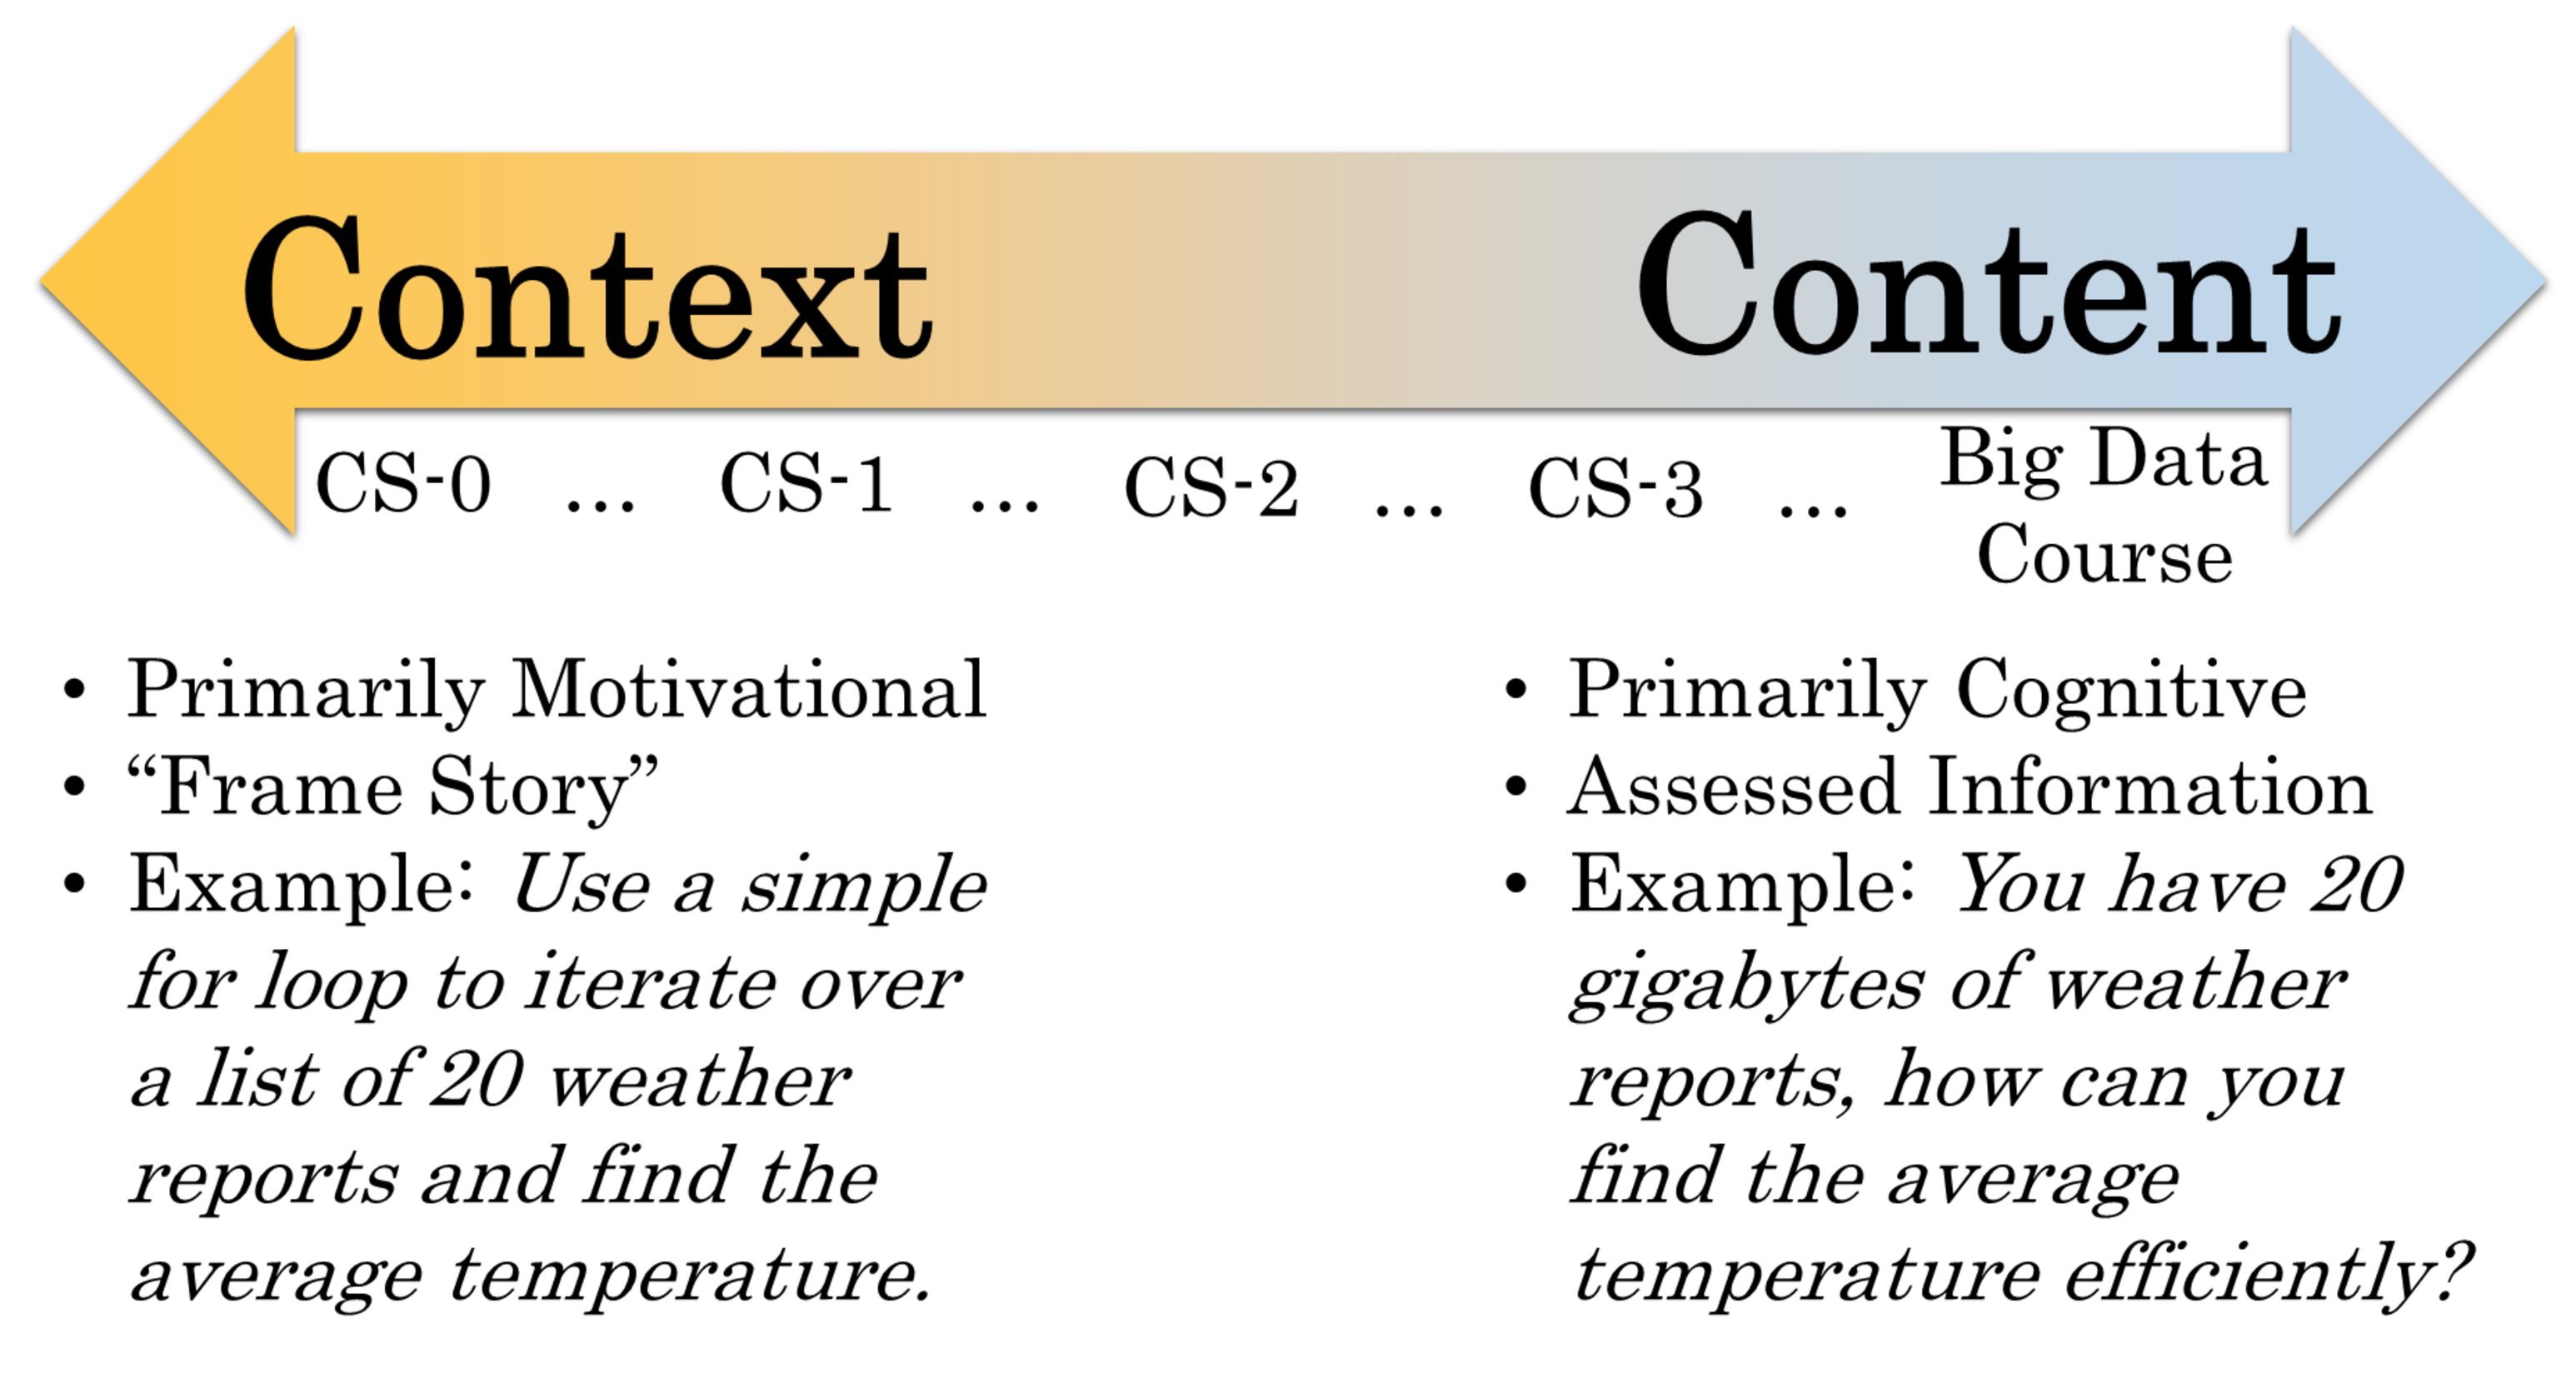
\psfig{file=images/content-context-2.eps, width=\linewidth}
		\end{center}
		\caption{Content vs. Context}
		\label{fig-content-context}
\end{wrapfigure}

\begin{description}
	\item[Context] ``... The problem's physical and conceptual structure as well as the purpose of activity and the social milieu in which it is embedded''\cite{rogoff1984everyday}, context is driven not just by the atmosphere of the problem at hand, but also by the background and culture surrounding the problem.
	A good context enables a student to find recognizable elements and build on prior understanding, eventually being able to freely transfer their learning to new contexts.
	\item[Content] The information intending to be conveyed to the students.
	If context is the backdrop to the learning, then content might be seen as the plot.
	Naturally, context and content are deeply intertwined with each other, and its difficult to talk about one without referencing the other; in fact, content is an abstract entity that needs to be made concrete through contextualization when it is delivered to the learner.
	If the information is too abstract, than it will never connect with the learner and will not be transferable to new domain.
	However, if it is too grounded in a domain, then it will not be clear how it can be re-applied elsewhere. 
	Ultimately, content must be given in a variety of forms to maximize transfer.
	Two useful methods for building content are anchored instruction (exploring scenarios, or anchors, in the context based on the content) and cognitive apprenticeship (mediating knowledge from an expert to the novice learner in a mentoring relationship).
	\item[Facilitations] The modifications to the learning experience that support and accelerate learning.
	Facilitations provide opportunities for students to internalize what they are learning by lowering the barriers that can surround situated experiences, possibly at the cost of some amount of authenticity. 
	These modifications might be technological in nature, but they can also be pedagogical.
	Although there are many different forms that Facilitations can take, Scaffolding is one of the most common.
	Scaffolding is a form of support that is intended to extend what a learner can accomplish on their own.
	This support is required at the onset of the learning process, but is unnecessary once a sufficient threshold has been passed; during this transition, the amount of scaffolding can be tuned to the learners understanding.
	In Computer Science, for instance, students often take advantage of software libraries and frameworks to create sophisticated graphical programs that would be beyond daunting if implemented from scratch.
	\item[Assessment] The methods used to assess the learning experience and the progress of the student.
	Choi \& Hannafin gives special attention to the “teach to the test” problem, and how assessment needs to change to measure students ability to solve authentic problem (as opposed to their ability to solve the test’s specific problem), and to be able to transfer their understanding when solving different but related problems.
	It is important that assessment is measured against the individualized goals and progress of a learner, requiring that any standards used be fluid and adaptable to different learners personal situations.
	Of course, assessment should be an on-going part of the learning process, providing feedback and diagnostics.
	Ultimately, the learner should join in the process of assessment as they transition to an expert – being able to meta-cognitively self-evaluate the effectiveness of ones methods and communicate results to others are key abilities of experts. 
\end{description}

There is a reciprocal relationship between contexts and content.
Figure \ref{fig-content-context} demonstrates an example of this relationship for the expected emphasis on big data as context vs. content throughout an undergraduate curriculum, from a CS-0 (non-majors) course all the way to an upper-level course specifically on big data.
Just as the upper-level course would naturally use big data as its context and content, a CS-0 course could still have content related to big data.
However, the majority of the use of big data would be as the framing story for assignments, especially in earlier parts of the course.
When students learn programming in the context of, say, game development, they are almost necessarily learning content related to game development that may not be universal to computer science -- e.g., how graphical resources are organized and accessed within the game engine.
This content may be seen as a distraction by the instructor, or as useful side knowledge - for example, if a student had to learn how to use a command line in order to compile their game, they would be learning an authentic skill that might not be considered part of the core content, but is nonetheless generally useful.
When evaluating a context, it is useful to consider what content it represents, and how authentic and useful it is.
The authenticity of content that is attached to a context affects the authenticity of the learning environment as a whole.

Fascinatingly, the need for a strong context diminishes as learners mature and become domain-identified -- the content itself becomes the context.
Learners start to see other contexts as nothing more than distractions and unnecessary fluff.
This makes sense -- you would hope that Computer Science majors in their third semester would be naturally interested in the material, and this is borne out in experimental data.
For instance, Yarosh \& Guzdial attempted to integrate Media Computation in a CS-2 (Data Structures) course, and found that the learners had ``outgrown the desire for a context''~\cite{yarosh2008narrating}. 
These results are similar to results we found in our interventions with a CS-3 (Data Structures and Algorithms), where students seemed more irked by the surrounding context than intrigued.

\begin{figure}
	\begin{center}
		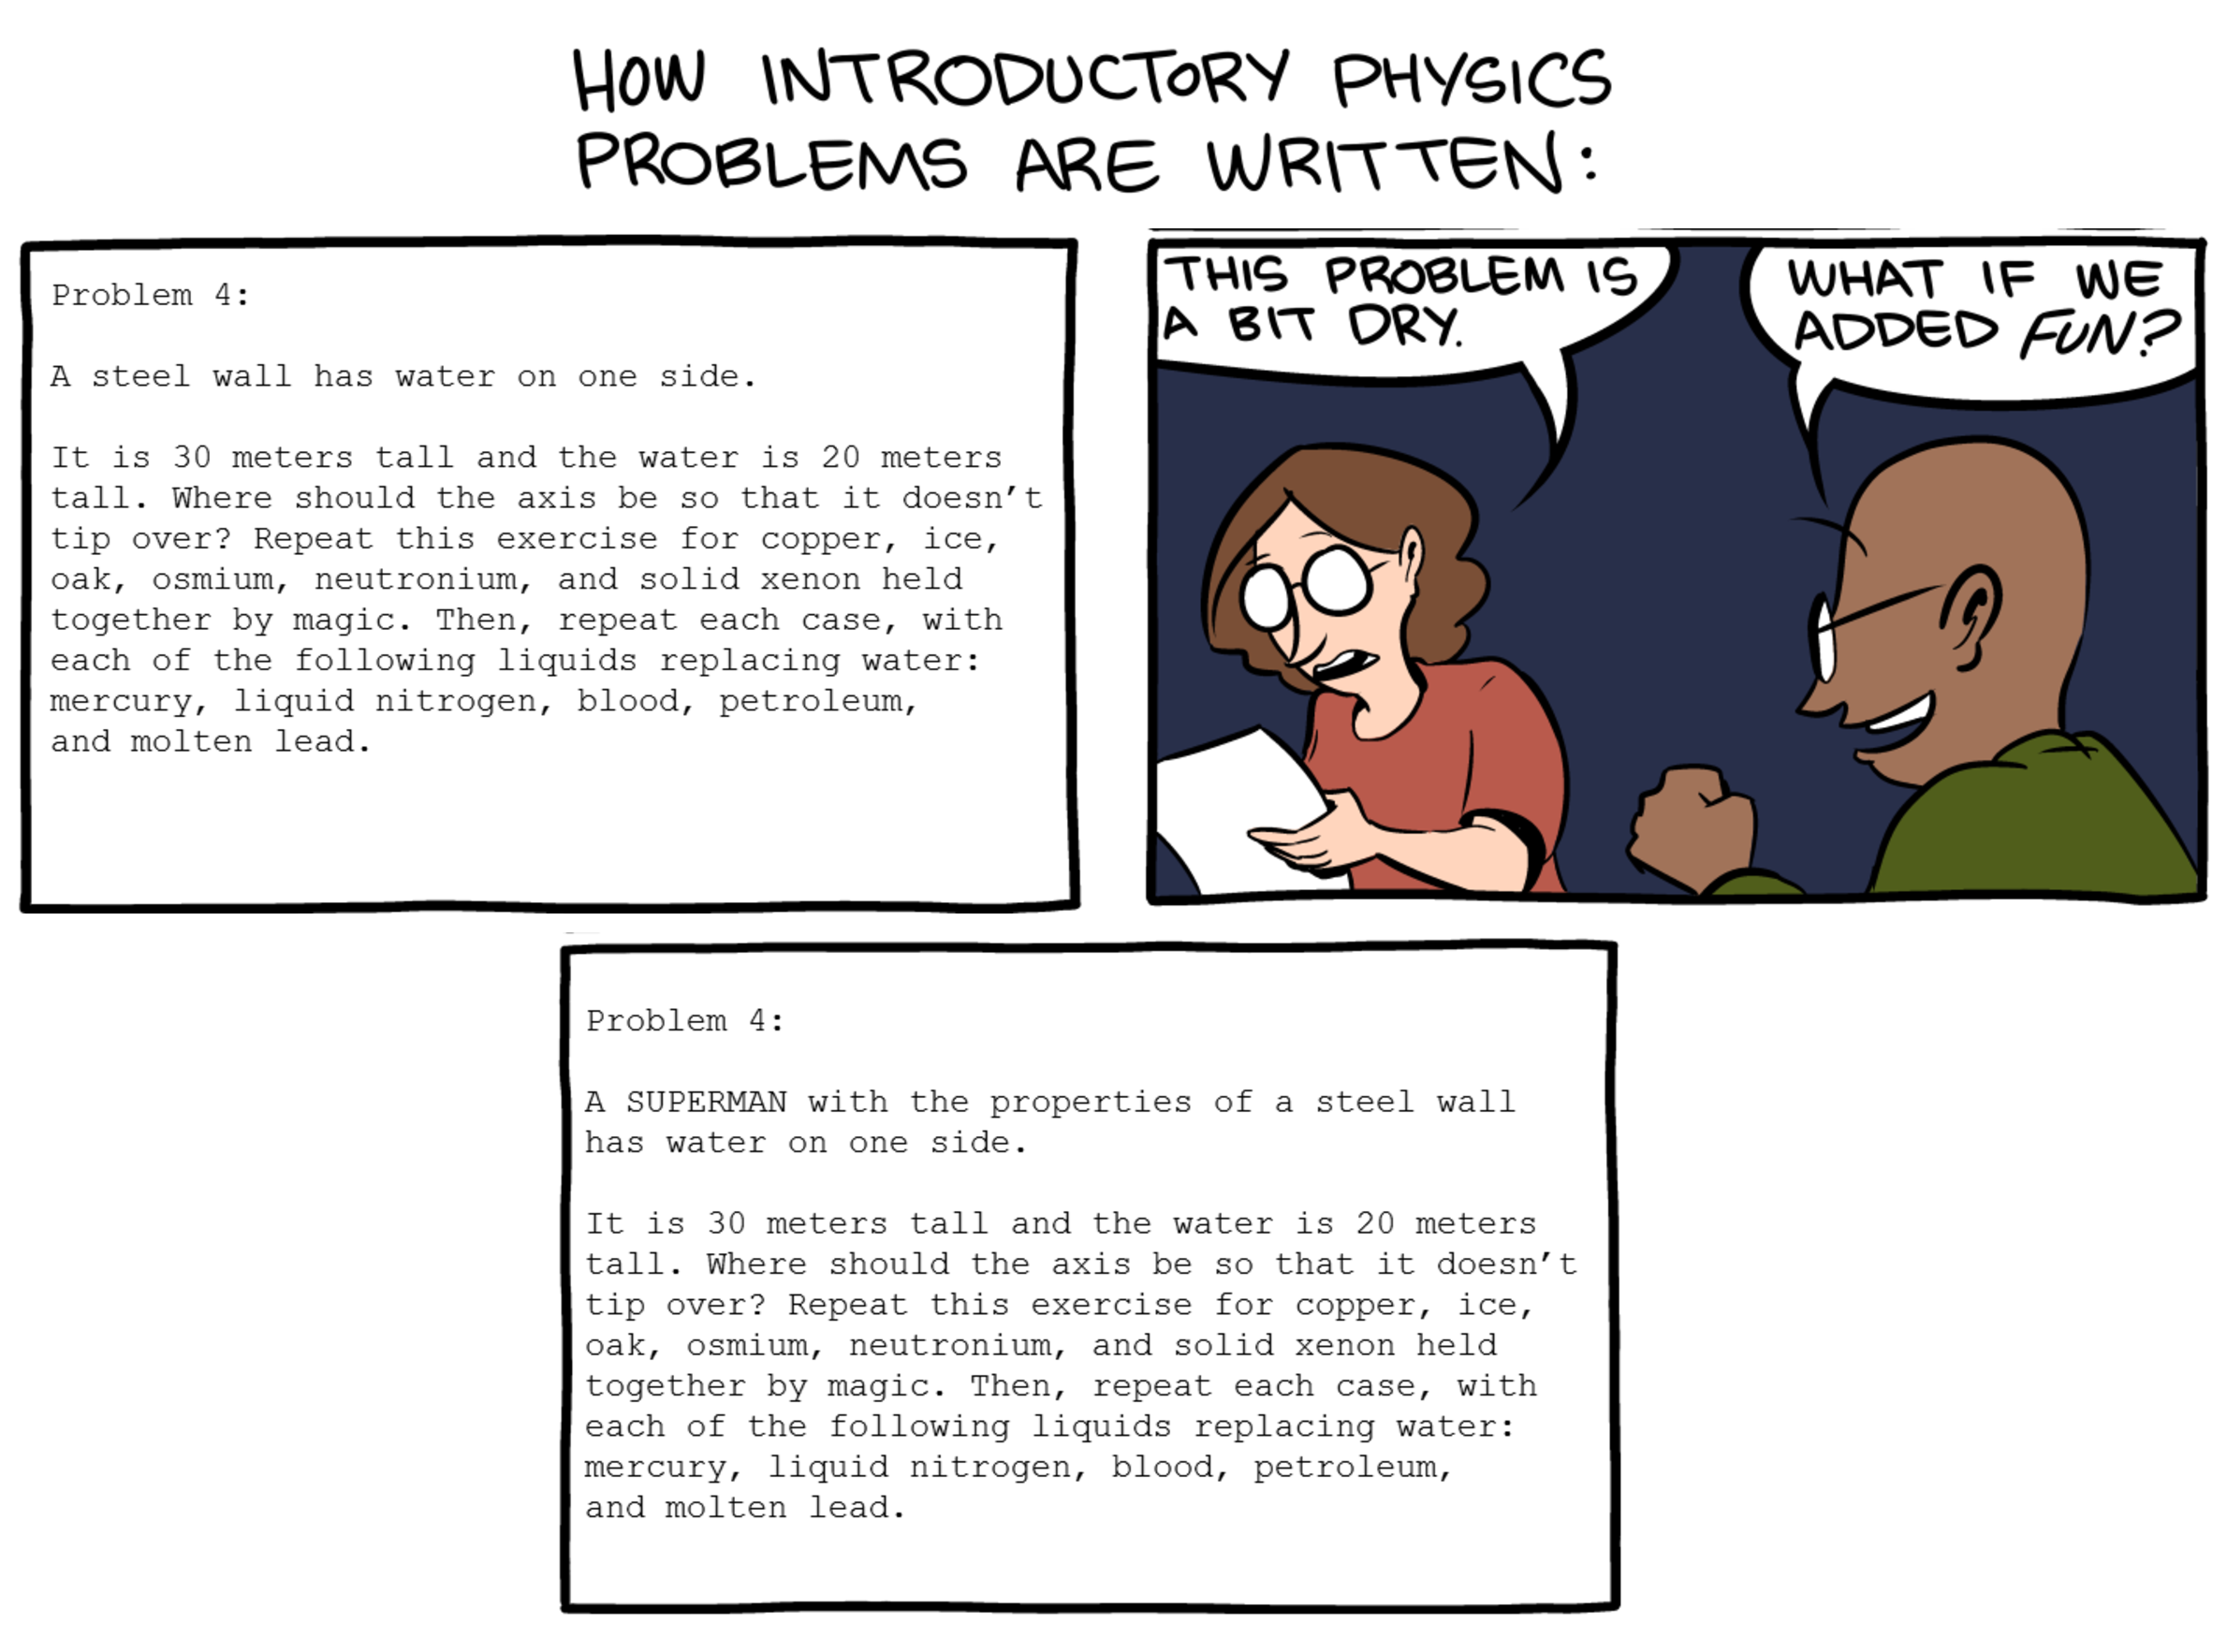
\psfig{file=images/smbc.eps, width=\linewidth}
	\end{center}
	\caption{Making the context ``Fun'' is not necessarily trivial, whether in physics education or computer science education.~\cite{SMBC}}
	\label{fig-comic-context}
\end{figure}

Of course, it is up to instructor to determine the depth and breadth of the context's integration.
The trade-off between the value and distraction added by the context is a delicate formula.
Consider the scenario in figure \ref{fig-comic-context}.
A steel wall is a relatively relatable concept for most students -- they can readily imagine such a large, durable object, and it somewhat reasonable to expect that objects would interfere with it.
In this scenario, the instructors consider replacing the wall with a comic book character -- something that they anticipate will be more ``fun''.
If they are in tune with their learners, this might actually be an effective context -- perhaps they know that their learners are comic book fans.
However, because the integration is only at the surface level, it is possible that the learners will see this as a forced reference, and they will have a more negative reaction.
It is also possible that they will not recognize the reference, or feel no positive emotions with it -- many contexts do not take into account gender, racial, or socio-economic characteristics of the anticipated learner.


\subsection{Theories of Motivation}

%TODO

\subsubsection{MUSIC Model of Academic Motivation}

Situated Learning is a theory of learning, but is not a comprehensive motivational framework -- it describes how people learn, but it is limited in explaining why people commit to learning.
Instead, it is useful to turn to the dedicated motivational models as a lens to explore why people choose to participate and excel in Computer Science.
In this preliminary proposal, we lean on the MUSIC Model of Academic Motivation as a primary framework.

The decision to use the MUSIC model was based on several criteria.
Although there are many motivational models available, few strive to be holistic models specifically developed for academics.
For example, theories like Expectancy-Value and Cognitive Evaluation Theory have a wider scope and have stemmed from other disciplines such as healthcare.
The MUSIC Model is derived from a meta-analysis of these other theories, incorporating only the academically relevant components.
Further, the MUSIC model is a tool meant for both design and evaluation, allowing it to be used in all phases of this work.
Finally, the model and its associated instrument, the MUSIC Model of Academic Motivation Inventory (MMAMI) , has been extensively validated and utilized in other educational domains, making it a reliable device\cite{jones-validity}.

The MUSIC model identifies five key constructs in motivating students \cite{jones-description}:
\begin{description}
	\item[eMpowerment:] The amount of control that a student feels that they have over their learning -- e.g., course assignments, lecture topics, etc..
	\item[Usefulness:] The expectation of the student that the material they are learning will be valuable to their short and long term goals. There is no clear delineation of the time-scale for these goals, but there is nonetheless a distinction between strategic skills that students need to be successful in careers and personal interests and the tactical skills they need to complete present-day tasks.
	\item[Success:] The student's belief in their own ability to complete assignments, projects, and other elements of a course with the investment of a reasonable, fulfilling amount of work.
	\item[Interest:] The student's perception of how the assignment appeals to situational or long-term interests. The former covers the aspects of a course related to attention, while the latter covers topics related to the fully-identified areas of focuses of the student.
	\item[Caring:] The students perception of other stakeholders' attitudes toward them. These stakeholders primarily include their instructor and classmates, but also can be extended to consider other members of their learning experience (e.g., administration, external experts, etc.).
\end{description}

Students are motivated when one or more of these constructs is sufficiently activated.
They are not all required to achieve maximal levels, and in fact that is not always desired -- it is possible, for instance, for a student to feel too empowered, and become overwhelmed by possibilities.
For some of these constructs, a careful balance is required, and it may not be possible to ever achieve a minimal level; no matter how exciting you make your lecture, you may never convince your students it is interesting, although it is possible that they will still consider it useful and stay motivated.
Much like in Situated Learning Theory, students' subjective \textit{perception} of these constructs is a defining requirement and is more important than objective reality.

The MUSIC model is often used as an organizational framework and an evaluative tool.
As the former, it is a list of factors to consider when building modules, assignments, and content of a course.
At all times, instructors can consider whether they are leveraging at least one construct to motivate their students.
As the latter, it offers both a quantified instrument (MMAMI) and a structure to anchor a qualitative investigation on.
The model has also directly been used tactically in course design: Jones describes a controlled classroom experiment to motivate students by having an experimental group reflect on how a course satisfies the constructs of the MUSIC model (e.g., prompted to answer ``How will the material presented here will be useful to you?'').
Quantitative data gathered after the experiment indicated a significant increase in motivation.~\cite{mcginley2014brief}

\subsubsection{Self-Efficacy}

Although the MUSIC Model is a holistic model, it can be useful to explore other theories of motivation that it draws on.
Self-efficacy is just such a theory, concerned with a learners judgment of their own capabilities.
Self-efficacy is often a strong predictor of students performance.
Students that believe they will fail will often do so, despite whatever ability they may have.

\subsubsection{Self-Regulation}
In the Self-Regulated Learning (SRL) model, learners succeed by actively practicing and developing their learning, willingly taking on challenging tasks, and reflecting on their strategies that lead to success.
In Computer Science, students must develop their understanding of how long programming tasks take, understand where their conceptual knowledge is weaker and believe that they can improve (as opposed to a fixed view), and a host of other meta-cognitive skills.
In an algorithms and data structures (CS3) course at Virginia Tech we have observed that students often have difficulty with the course programming projects.
These projects involve concepts such as dynamic memory allocation, recursion, file processing, differing interpretations of the bytes that represent data, and a collection of interacting classes.
The designs are more complex than students are used to, as the projects stress interacting classes requiring appropriate separation of concerns.
Too large a fraction of these students are unable to properly manage their time.
Research on procrastination [18, 19] indicates that motivation and self-efficacy for time management are key determinants for avoiding procrastination. In this project, we will provide big data as an available source of "inter-esting" projects.

\subsubsection{Extrinsic Motivation}

Although ideally, students will always be internally motivated to learn new subjects, this isn't always the case.
Academics are a careful balance of extrinsic and intrinsic motivation, with both internal and external rewards.
For instance, the ultimate goal of most formal education is certification, either by an accredited university or some other independent body.
In order to keep students on task, positive and negative grades are assigned based on performance.
Although these grades can drive negative behavior (e.g., nit-picking, arguments, etc.), they are ultimately necessary for some class of learners.
It can be a serious challenge for instructors to assign grades and use other forms of extrinsic motivation, to avoid dragging students along in a rigid environment but also not preventing students from floundering.
Too loose with a grading scheme, and students may deprioritize a course over stricter ones.
Too hard, and students may feel overwhelmed.
Although my research will not focus much on extrinsic motivation, it is important to understand its role in the classroom experience.
    \section{Introductory Computing}

In the following sections, we review existing literature on the many forms that introductory computer science has taken.
This is not intended to be an exhaustive look at all the ways to teach Computer Science.
Instead, it will be illustrative of the many approaches that the community has been exploring over the past few decades, along with the successes and failures of the different approaches.
It will begin with a look at what content should be taught and who should receive the instruction.
Then we will explore the approaches and tools that have been used to mediate the instruction and, finally, the assessments used to measure the success of the approaches.

\subsection{The Content}

There is a serious, on-going debate about what novice students in computing should learn, with limited consensus. 
Complicating this discussion is the bifurcation of introductory computing into Computational Thinking (sometimes referred to as CS-0) and Computer Science (sometimes referred to as CS-1).
At the same time, both of these pathways claim to be ``more than just programming.''


\subsubsection{Programming}

Programming is the process of writing explicit instructions, executable by a computational agent, to solve a seemingly-infinite number of computationally-susceptible problems, such as summing large lists of data, processing and rendering images, or creating complex interactive media. Programmers write instructions to the computer that will be executed on command, instructions that come in a variety of forms called \textit{languages}. These sequences of instructions, programs, were originally hard-wired into the machinery of a computer, but are now created using programs called \textit{programming environments}. Today, these environments are arguably the primary tools of a developer, and are where both experts and novices spend the majority of their time. The learning environment of a programmer, therefore, are these programming environments.

\subsubsection{Computer Science}

Computer Science is often described as neither being about Computers, nor being a science.
Instead, it is a complicated blend of engineering, science, art, and several other disciplines.
It attempts to solve problems using computation, finding what is theoretically computable and what is not, and many other complicated tasks.
A full description of what Computer Science is and is not is outside the scope of this proposal.
Computer Science Curriculum 2013 \cite{CS2013} is an attempt to codify the entire breadth of an undergraduate CS education.
However, it does not attempt to dictate the exact implementation and order of material.
Traditionally, certain topics are typical -- decision, iteration, and the nature of data and control flow.

Different curriculums, therefore, suggest different approaches.
The ``How to Design Programs'' curriculum emphasizes a functional programming model, using a LISP-descended language named Racket.
The only looping mechanism that students are taught is recursion.
The dominance of the Object-Oriented Model in software engineering usually leads to a strong emphasis in introductory courses -- in fact, there is even an ``Objects First'' curriculum.
There are other approaches, of course -- some instructors focus on an initially imperative programming style, to focus on high level concepts such as program state and coding instructions.

\subsubsection{Computational Thinking}

In the past few years, there has been a push for "Computational Thinking" in curriculums outside of Computer Science. 
The phrase was coined by Seymour Papert in 1993~\cite{papert1996} and popularized by Dr. Jeannette Wing's 2006 paper~\cite{wing2006}, which opened a floodgate of discussion about the term. 
Unfortunately, there is still limited consensus on \textit{what} exactly CT is, whether it should be universally taught, how it should be taught, and how to identify when it has been taught.

An excellent resource for summarizing the history of Computational Thinking research is the 2013 dissertation by Wienberg~\cite{weinberg2013}. 
This comprehensive survey analyzed 6906 papers directly or indirectly related to Computational Thinking from 2006-2011, describing research efforts and findings. 
Those papers were filtered down to 164 papers that substantially related to Computational Thinking in order to draw more meaningful conclusions. 
Finally, 57 of these papers were given closer treatment to analyze their research methods.

Weinberg paints an interesting picture of Computational Thinking research. 
As might be expected, there has been a steady increase in published papers on the topic since 2006.
The movement is focused in the US, with less than a quarter of first-authors being outside the United States, even though 55\% of Computer Science research (beyond just Computer Science Education research) is published outside of North America~\cite{Randolph2008}. 
Research is divided evenly between K-12 and undergraduate, and there is no strong presence of research on continuing or post-graduate education initiatives that involve Computational Thinking.
    
An important contribution by Weinberg is a taxonomic breakdown of the aforementioned 164 research papers based on whether they primarily focus on modeling, pedagogy, or assessment. 
This taxonomy is documented in Appendix \ref{app:weinberg-taxonomy}, and a summary of the results of this breakdown is shown in Figure \ref{weinberg-taxonomy}. 
Over half of the research on CT describes approaches to pedagogy (Curriculum and Program Description), leaving a small amount to modeling (Philosophy and Opinion) and assessment (Research and Evaluation). 
The lack of assessment research is understandable given the youth of this area of research, but still troubling.

\begin{figure*}[h]
    \centering
		
		\def\angle{90}
		\def\radius{3}
		\def\cyclelist{{"deepred","red","deepgreen","green","deepblue","blue"}}
		\newcount\cyclecount \cyclecount=-1
		\newcount\ind \ind=-1
		\begin{tikzpicture}[nodes = {font=\sffamily}]
			\foreach \percent/\name in {
					48/Curriculum Description,
					7/Program Description,
					12/Research,
					5/Evaluation,
					23/Philosophy,
					6/Opinion
				} {
					\ifx\percent\empty\else               % If \percent is empty, do nothing
							\global\advance\cyclecount by 1     % Advance cyclecount
							\global\advance\ind by 1            % Advance list index
							\ifnum5<\cyclecount                 % If cyclecount is larger than list
								\global\cyclecount=0              %   reset cyclecount and
								\global\ind=0                     %   reset list index
							\fi
							\pgfmathparse{\cyclelist[\the\ind]} % Get color from cycle list
							\edef\color{\pgfmathresult}         %   and store as \color
							% Draw angle and set labels
							\draw[fill={\color!50},draw={\color}] (0,0) -- (\angle:\radius)
								arc (\angle:\angle+\percent*3.6:\radius) -- cycle;
							\node at (\angle+0.5*\percent*3.6:0.8*\radius) {\percent\,\%};
							\node[pin=\angle+0.5*\percent*3.6:\name]
								at (\angle+0.5*\percent*3.6:\radius) {};
							\pgfmathparse{\angle+\percent*3.6}  % Advance angle
							\xdef\angle{\pgfmathresult}         %   and store in \angle
						\fi
					};
			\end{tikzpicture}
    \caption{Percentage of Papers in Each Category of the Weinberg Taxonomy}
    \label{weinberg-taxonomy}
\end{figure*} 

Even more troubling, however, is the further analysis of the 57 empirical studies.
Only fifteen (26\%) studies include or sought an operational definition of computational thinking, and only six go beyond the superficial (solely describing computational thinking as a "way of thinking", a "fundamental skill", or a "way of solving problems"). 
The failure to identify an operational definition weakens the theoritical strength of the studies.
This weakness likely stems from the background of the researchers: 28\% of the articles involved non-CS majors and \textbf{only 18\% of the articles involved education experts.} 
In other words, over four-fifths of this educationally-oriented research was performed by people with no real formal training in educational research techniques.
This is particularly troubling given that Computational Thinking is a strong target for interdisciplinary endevaors.

Weinberg reflects on the continuing debate about the importance of Computational Thinking:
\begin{quote}
    Many, like Wing, believe computational thinking to be a revolutionary concept, one as 
important to a solid educational foundation as are reading, writing, and arithmetic (Bundy, 2007\cite{bundy2007}) 
(Day, 2011\cite{day2011}). Others believe its potential and significance are overstated (Denning, 2009\cite{denning2009}; 
Hemmendinger, 2010\cite{hemmendinger2010}), and some have voiced concern that by joining forces with other 
disciplines computer science might be diluting either one or both of the participating disciplines 
(Cassel, 2011\cite{cassel2011}; Jacobs, 2009\cite{jacobs2009}). Both the praise and the criticism for computational thinking could 
perhaps be tempered by reflecting on a historical quote by Pfeiffer in 1962: “Computers are too 
important to overrate or underrate. There is no real point in sensationalizing or exaggerating 
activities which are striking enough without embellishment. There is no point in belittling 
either.” (Pfeiffer, 1962\cite{pfeiffer1962}).
\end{quote}

Computational Thinking often strives to teach more than just the practical mechanics of programming and Computer Science.
Instead, it is suggested as a set of cognitive techniques, such as iterative design, a debugging mindset, and more.
Philosophers often also describe ``dispositions or attitudes'' that a computational thinker should exhibit\cite{csta-computational-thinking}:
\begin{itemize}
\item Confidence in dealing with complexity
\item Persistence in working with difficult problems
\item Tolerance for ambiguity
\item The ability to deal with open ended problems
\item The ability to communicate and work with others to achieve a common goal or solution.
\end{itemize}
Though defined for K-12 education, these dispositions seem equally relevant to university-level students. The first four dispositions influenced our use of student-defined big data projects where complexity, difficulty, ambiguity and open-endedness are present. The last disposition influenced our use of multi-disciplinary cohorts.

There are key differences in these two educational pathways (Computer Science and Computational Thinking) that strongly influence course design.
First, Computational Thinking courses are usually terminal and intended for non-majors -- there is little-to-no expectation that they will take more Computer Science courses.
By comparison, CS-1 is a foundational course meant for students majoring in Computer Science.
Typically, expectations are lower for students in CS-0, and less material is covered -- critically, there is a reduced emphasis on programming in favor of higher level concepts.
Many students that try to transition from CS-0 directly to CS-2 will struggle, and it is still unclear how these students can be brought to success.

Regardless of the differences between these different subjects, it is clear that both Computational Thinking and Computer Science rely on programming to some degree, and some degree of the subject must be taught before these students will really succeed with the rest of the material.
Although Computational Thinking is more than just programming, it is still a crucial element.

\subsection{The Learners}

In any instructional design model, a crucial task early on is to identify the audience of the instruction -- what their backgrounds are, their motivations, their abilities, and their goals.

The most obvious audience for instruction on introductory computing is undergraduate computer science majors -- the ones who come to college explicitly to learn computing. 
These students often have already had prior successful computing experiences -- either in high school AP courses or through their own side-projects.
However, some large percentage of students typically enter without any prior experience, and are overwhelmed by the material and the gap between themselves and their more experienced peers.
Harvey Mudd has had great success in separating these two classes of learners to improve the introductory computing experience.~\cite{Alvarado:2010:WCE:1734263.1734281}

Recent efforts have started to push introductory computing into lower grades, i.e. K-12.
Younger students tend to have less fully defined domains, which means that it is more important to rely on situational interests and short-term expectations of usefulness.
These students also have a weaker overall cognitive base to draw on, necessitating simpler materials.
However, this can be an advantage for students, as it represents a level playing field.
Of course, the imbalance of computational resources (e.g., computers) across the world can make it difficult to provide meaningful experiences for these students.

A final categorization is non-majors taking Computational Thinking, a primary target of my research efforts.
These students present a unique profile.
A few of them will have had prior programming experience, but most of them have had very minimal interactions with computers (indeed, some will describe themselves as ``not a computer person'').
These students may not believe that Computational Thinking will help them.
This is largely because they have more clearly defined domain identities, and may not see how Computational Thinking fits into them.
So, indeed, these students often have low motivation and low ability.

\subsection{The Contexts}

As part of the overarching goal to bring more students into Computer Science, a large number of contexts have been explored in Introductory computing. 
The context of a learning experience grounds the learner in what they already known, in order to teach the new material.
Many introductory computing experiences focused on presenting the content as purely as possible, which can come across as abstract and detached~\cite{Zografski}.
However, starting with Seymour Papert's work with robotics and the LOGO programming environment in the 70s~\cite{papert1996}, instructors have been interested in motivating students' first experience with rich contexts.
Two particularly popular approaches have emerged since then -- Digital Media ``Computation'' (Manipulation)~\cite{Forte} and Game Design~\cite{Zografski}.
However, an alternative approach that is steadily gaining popularity is [Big] Data Science ~\cite{Anderson}.



\subsubsection{Interest-Driven Contexts}

As it became clear that Computer Science had a serious image problem (Denning describes its perception by the public ``stodgy and nerdy''~\cite{Denning:2005}), work began on making Computer Science ``Fun'' and approachable. 
A key goal was to increase diversity and to broaden participation. 
This led to the rise of ``Interest-Driven Contexts'', emphasizing problems and projects that would be situationally interesting to a wide audience.
Guzdial, for instance, was largely responsible for the creation of the Media Computation approach, where students use computational techniques (e.g., iteration and decision) to manipulate sound, images, videos, and other digital artifacts.
For instance, students might use a nested, numerically-indexed \texttt{for} loop in order to adjust the red-value of the pixels in an image, treating it as a two-dimensional array of binary triples, in order to reduce the red-eye of a photo.

Although wildly deployed, a review of these curricular materials by Guzdial \cite{guzdial2006imagineering} in light of Situated Learning Theory found that 1) students did not find this an authentic context, and 2) intense rhetoric was insufficient to convince them that it was authentic. 
Few students find it expedient and helpful to remove the red-eye from family photos by writing python scripts, when they could easily use a GUI-based program to automate the task instead.
Guzdial leaves open the question of what contexts can be truly authentic for non-majors, given the relative novelty of teaching introductory computing for non-majors.
Ben-Ari echos this question by suggesting a very narrow selection of authentic contexts and communities in his paper exploring the application of Situated Learning Theory to Computer Science in general \cite{ben2004situated}.
Critically, the opposite problem could occur -- if an instructor is effective at convincing students a context is authentic, they may believe them.
There are serious ethical issues involved in mispresenting the utility of a context, leading students to develop an embarrassing misconception of the field -- imagine a young child believing that all of Computer Science is game design, because that is what they started off doing.

There are other disadvantages of an Interest-driven approach.
The motivation literature describes ``Seductive Details'' (interesting but irrelevant adjuncts)~\cite{harp1998seductive} as interfering both with short-term problem completion and long-term transfer.
In other words, students get hung up on unimportant aspects of the context that they ignore the content.
Consider a student using the game and animation development environment Scratch, which allows beginners to create sprites from images.
A young learner may be so amused by the ability to change the color and shape of their image, that they neglect their assigned work.
Although a well-regulated learner would not be distracted, most of the at-risk population that would benefit from these contexts are unable to deal with such distractions.

\subsubsection{Useful-Driven Contexts}

An alternative focus to Interest is Usefulness, the idea that the context should be immediately authentic to the learner.
To some extent, it is impossible (or at least prohibitively difficult) to find a one-size-fits-all context that will be useful to all learners.
To do so could be considered preauthentication.
However, in practice, some contexts are broadly useful that they are likely to engage a diverse crowd of learners, and simultaneously providing opportunities to empower the learners.
Perhaps the most open-ended and valuable context is pursuing real-world problems across many different domains.

In the past two decades, the field of Data Science has emerged at the intersection of Computer Science, Statistics, Mathematics, and a number of other fields.
This field is concerned with answering real-world problems through data abstractions.
As a context, there are pedagogical penalties for using it, since it introduces a wide variety of new content -- visualization, statistics, ethics, social impacts... the list is long.
However, a good instructor can downplay the focus on these side-areas as needed, or even emphasize subject matter's strengths (e.g., a statistics major might find it interesting to use their mathematical background to strengthen their problem-solving investigation).
However, there are other difficulties: bringing in real-world data requires real sophistication by the instructor, especially when working with Big Data.

The use of data analysis as a form of contextualization is not novel, and represents a new and actively growing movement.
Recently, low velocity and low volume data sets have been provided by Anderson et al to explore interesting questions in CS-0 courses \cite{Anderson}, building on a small history of similar projects.
Typically, these questions are provided as uniform experiences for the students in the course -- everyone works with the same dataset.
Upper division courses have employed these situated learning experiences using data of varying size and complexity for several years \cite{Egger, datamining, Waldman}.
Many authors collaborated to produce a new framework centered around these ideas -- ``Social Computing for Good'', a collection of approaches and projects for interdisciplinary students to solve using computing ~\cite{Social-good}.
Although this framework presents some ideas, there are still unsolved technical and pedagogical problems in how to optimally bring these materials to learners.

\subsection{The Facilitations}

The faciliations of a learning experience are the scaffolds used to support the learner, which must eventually be faded away as they progress.
Although in an ideal experience, the learner will complete all materials with no more support than an expert, in practice they often need help getting started.
Many such tools have been created to support computer science education over the years.
Some of these tools have a deep integration into the learners environment  -- which is typically a programming environment.
Programming environments are an integrated tool for programmers to write, execute, and debug code.
There are many, many programming environments out there, and many have been designed with learners in mind (e.g., Dr. Racket, Greenfoot, Scratch, etc.).
This section describes some common tools and ideas that are used in CS Education - it is meant to be more illustrative than exhaustive, but highlights the primary technological means that are used to support learners.

\subsubsection{Block-based Programming}

A historically successful approach to gently introducing students to programming is block-based programming, such as Scratch and its successor Snap!.
These environments introduce high-level programming concepts by having students connect blocks representing programming constructs in order to avoid syntactical barriers -- grammatically-incorrect combinations are forbidden by the design of the system.
Although equivalent in computational power, block-based languages have long been known to be unsuitable for professional developers because of their failure to scale and their inflexibilty. 
And yet, instructional design dictates that the learning context should match the performance context as closely as possible to ensure transfer.
Therefore, a recent criticism of this approach is that transferring students from a block-based language to a traditional text-based language is a non-trivial problem that must be studied closely.

\subsubsection{Visual Programming Environments}

Another common facilitation is Visual Programming, which features images as a principle component of the process of abstraction.
Students struggle with the idea of ``abstraction'', representing complex real-world phenomenon with simplified representations.
Although an expert computer scientist is comfortable treating today's weather as a single number, it can be challenging for a beginner to separate out the complexities and mentally model the computer's knowledge.
Visual Programming seeks to alleviate this problem by definitively including image information along with the representation -- and by extension, also including position, shape, color, etc.
This can be extremely effective for agent-based systems (e.g., NetLogo~\cite{tisue2004netlogo}) and game/animation environments (e.g., GreenFoot~\cite{Kolling:2010}).

A major trade-off of such a system is that students become dependent on the images as a crutch, and believe that an image is a necessary component of the representation process.
They will still eventually have to deal with abstract ideas that do not necessarily have pictoral representations -- ``Manager'' style classes that drive more abstract components of computation often have suffer from such a challenge.
Some systems incorporate an ethereal construct -- NetLogo has the idea of ``Observers'', which can help students adjust to the idea.

\subsubsection{``Run'' Buttons}

Compiling and running a program is a multi-step process -- a consummate computer scientist should have an awareness of how the system translates and links the high level code into a format runnable by the system.
Many low level programming languages demand the user interact with it through a command line, in order to take advantage of all the configurations it demands.
Modern programming environments often hide all of this complexity away with a simple ``run'' button.
In some cases, this is further abstracted by hiding the concept of a ``main'' function -- e.g., in GreenFoot, students define behavior for objects through a special class hook, and the system is responsible for executing these objects according to its own schedule.
Insulating from the command line hides ``real programming'', and this may affect students' perceptions of the systems' authenticity -- an instructor may also consider it insulation from crucial knowledge on how a program should be run, and the messiness that can be involved in the process.

\subsubsection{Program Analysis}

Modern environments often perform some kind of analysis of a program in order identify flaws, whether syntactical, stylistic, or semantic~\cite{Ihantola:2010}, providing automated guidance to the learner.
The latter-most of these is a true challenge that requires the instructor to provide additional information to the system (e.g., unit tests and program constraints).
The former are more straight-forward, and have broad application to programming.
Program analysis is a complicated process that combines static parsing of programs (often using type information) and dynamic analysis (requiring the system to be run).
The Unit Testing approach has led to the popularity of Test-driven development~\cite{webcat}.

\subsubsection{Program Visualization}

Beginners often struggle with understanding the idea of Program State, that a computer has a model that changes over the lifetime of a program.
Some environments and external tools can create visual representations of this state by executing an algorithm line-by-line.
For instance, the Online Python Tutor~\cite{Guo:2013} can map every line of code to an image representing the current stack and heap. 
Astute beginners can use this to explore how an individual statement affects the state of the system and to diagnose problems in their code.

\subsection{The Assessments}

A critical component of the educational process is assessment, both formatively to support the learning process and summatively to evaluate the students' (and research projects) success.
The Instructional Design process dictates that assessment tools align strongly with the high level performance objectives, requiring instructional designers to know what behaviors, skills, attitudes, and knowledge they expect of their students.
Different learners have different end-goals, and therefore require different measures of success.
For example, Computer Science students need to have a strong knowledge of how to program and solve certain kinds of problems; meanwhile, Computational Thinking students have lower requirements towards their knowledge of programming, but need to have a clear idea of how to apply what they know to their own fields' problems.

In an important retrospective paper, Guzdial listed and reviewed four hypotheses being measured by the Media Computation curriculum, evaluating whether the goals of the project were being met~\cite{Guzdial:2013:EHM:2493394.2493397}.
\begin{description}
	\item[Retention Hypothesis] Did more students stay in the course because of the new curriculum?
	\item[Gender Hypothesis] Were more women and other minorities retained and report higher engagement?
	\item[Learning Hypothesis] Did students learn more?
	\item[More-Computing Hypothesis] Did students choose to continue their study of Computer Science (e.g., by taking more classes or trying online curriculums)?
\end{description}
By evaluating the project against these hypotheses, Guzdial was able to do more than just identify the strengths and weaknesses of the Media Computation curriculum - he was able to identify weaknesses and strengths in his research approach.
For instance, Guzdial criticized the project for measuring absolute learning outcomes, rather than measuring learning gains for individual students -- pre- and post- tests are more reliable indicators of performance than only post- tests.
The lesson from this is that it critical to identify early and often what you are trying to assess and how it will be assessed.

\subsubsection{Performance Context}

Instructional Design dictates that assessment should be driven by the performance context.
However, the young and diverse nature of Computer Science and Computational Thinking make it difficult to narrow down what the performance context is.
Therefore, we take advantage of the context in order to solidify the performance context as the formalization of a problem, the abstraction of data related to the problem, and the creation of an algorithm to solve the problem.
This high-level goal contains several components -- most importantly, however, is that the goal is wrapped up in the idea of an algorithmic representation of a solution, necessitating students to write some code.

\subsubsection{Assessment Tools}

Given the goal, how do we assess success in introductory computing?
Expert programmers often measure the correctness of their programs using Unit Tests -- each individual unit of source code (such as a function or object, depending on the paradigm of the language) is given sample data along with the expected, correct output.
These unit tests can be run constantly during development to assess the ongoing validity of the code.
In some ways, these are simple measures of student success, and the test-driven development methodology has taken off to the point that one modern language, Pyret\footnote{\url{http://www.pyret.org}}, requires that all functions be written alongside its unit tests before it will even compile.
And yet Unit Tests are limited measures of achievement in the view of Situated Learning, which advocates for more active measures such as performance assessments.

Projects can be seen as a more authentic form assessment, and is suggested heavily by Situated Learning Theory.
Although projects introduce a considerable amount of complexity,
Evaluating a project requires some level of recital (e.g., by the student to an instructor) and can be graded against a rubric.
Of course, such measures can introduce a significant amount of bias -- care must be taken while developing the rubric in order to ensure reproducibility and reduce variance as instructors review the material.

Other aspects of Computational Thinking and Computer Science can be assessed with simpler instruments.
For instance, verbal information can be judged using a multiple choice examination, short answer questions, and other simplistic question types (e.g., matching programming constructs to their definition).
Intellectual skills such as iterating over data can be tested with short programming exercises.
More complicated conceptual knowledge can be evaluated by requiring the students create concept maps and paragraph responses.
However, generalized, repeatable concept inventories remain an elusive prize for Computer Science educators, although Tew and Guzdial~\cite{Tew:2011:FLI:1953163.1953200} have had some measure of success.


    \section{Big Data Science}

Big Data is much in the news these days, from reports of massive data
dredging by the NSA to tens of millions of credit cards stolen by
hackers from commercial databases.
Big Data has become crucial to scientific advances from understanding the
genome to predicting climate change.
Unfortunately, computer scientists in the workforce are woefully
unequipped for this shifting paradigm.
Indeed, a report by MGI and McKinsey's Business Technology Offices
declares that ``by 2018, the United States alone could face a
shortage of 140,000 to 190,000 people with deep analytical skills as
well as 1.5 million managers and analysts with the know-how to use the
analysis of Big Data to make effective decisions.''\cite{McKinsey}
There are many obstacles to effectively educating students on Big
Data.
Its representation, manipulation, and expression is
challenging, with modern curriculums and programming tools being
inadequate.

\begin{wrapfigure}{r}{0.5\textwidth}
    \begin{center}
		    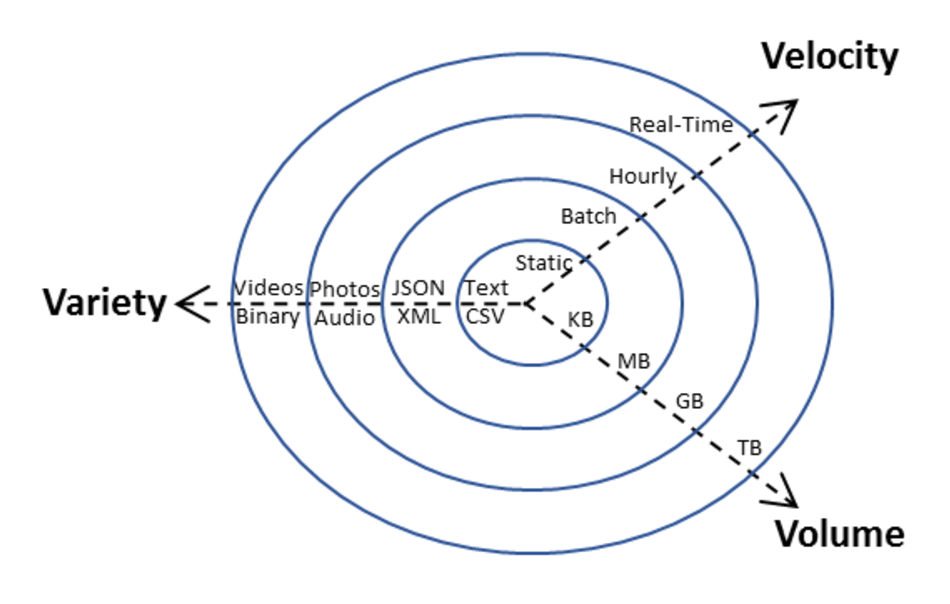
\psfig{file=images/3v-model.eps, width=\linewidth}
    \end{center}
    \vspace{-\bigskipamount}
    \caption{The 3V Model of Big Data}
    \label{fig-3v}
\end{wrapfigure}

Big data has been loosely described as quantities of information that cannot be handled with traditional methods ~\cite{McKinsey}.
But ``traditional methods'' is a vague phrase that has different meanings to different learners. To a Humanities major in their first CS-0 course, the traditional method to sum a list is to use Excel. In this scenario, ``big data'' means anything that won't comfortably fit into Excel's working memory.
However, to a third-year Computer Science major, the traditional method would be to write an iterative or recursive sequential loop; being given big data forces them to explore parallel models of execution.
Clearly, ``bigness'' is a function of the learner's experience, but that is still not a solid definition.

A more precise definition is the ``3V Model'' \cite{douglas2012importance}, which posits that there are three dimensions that distinguish big data from ordinary, run-of-the-mill data:

\begin{description}
	\item[Volume:] The total quantity of the information, usually measured in bytes or number of records. However, this also extends laterally: the number of fields in the structure of the data also impacts the complexity and size. The threshold at which data becomes big is a function of the hardware and software being used -- for instance, embedded systems may consider gigabyte-sized files to be big, while modern servers might not struggle until the petabyte level.
	\item[Velocity:] The rate at which new information is added to the system. High velocity big data implies a distributed architecture, since new data must be arriving from somewhere. The dynamicity of data can vary widely across these architectures, with data updating every year, every day, or even multiple times a second.
	\item[Variety:] The format or formats of the data. Ideally, data are always distributed in a way that is readily accessible -- for instance, simple text-based formats such as CSV and JSON are widely supported, relatively lightweight, and human-readable. More sophisticated data formats for image and audio are also typically well-supported, although still more complicated. However, projects using specialized, compressed binary formats or, more dangerously, multiple formats (e.g., image archives organized with XML files), are more complex.
\end{description}

In the remainder of this section, I describe common challenges associated with different kinds of data.

\subsection{High Velocity Data}

It is not trivial to enable introductory students to work with high velocity data, which is necessarily distributed. Without any scaffolding, it is necessary to delay the use of such data until much later in the course. In a prior paper \cite{realtimeweb-splashe}, we outline the biggest barriers to high velocity data as a context:
\begin{description}
  \item[Access] The process of programmatically downloading and parsing a web-based resource is a non-trivial procedure requiring an understanding of both basic concepts (e.g., function calls, data transformation) and specialized web technology (e.g., the difference between GET and POST calls, building query parameters).
	\item[Non-Idempotency] Because high velocity data is constantly changing, repeated calls to the same URL endpoint can return wildly different results, even over the course of a few minutes. This makes finding errors and testing considerably harder.
	\item[Consistency] Web-based APIs are controlled and developed by independent entities, which means that changes can occur at any time with little to no notification or time for reaction. This means that students' code can become out of date even during the middle of testing their final project.
	\item[Connectivity] Although internet speeds for students on a university campus are typically stable, this does not extend to off-campus students or students that are traveling. If the internet connection is down, then students might be completely unable to make progress.
	\item[Efficiency] Even when the internet connection is stable, it might not always be fast. Requiring a round-trip to a server can greatly drag on the testing and development process, frustrating the student and decreasing the time spent learning.
\end{description}

\subsection{High Volume Data}

In this section, we highlight some of the more challenging aspects of introducing high volume data, similar to how we previously outlined the challenges of high velocity data.
Some of these challenges are technical in nature, and some of them of a more pedagogical nature.
These challenges lead to certain design requirements that must be satisfied in any scaffolding intended to introduce high volume data.

\begin{description}
	\item[Data Transmission:] Internet connections can be difficult and inconsistent, especially for off-campus
and non-traditional students. Although most modern universities boast impressive wired connection
speeds, these speeds rarely extend off-campus. And even when internet connections are top-notch,
they can still be inadequate to serving the needs of transmitting big data collections to an entire
classroom of students. Some affordances must be made to make the data readily available to students without taxing their hard drives unnecessarily.
	\item[Different Contexts and Problems]: Additionally, high volume data offers different contexts and problems than high velocity data.
For instance, high velocity data typically lends itself to small quantities of data that are relevant to the current state of the real world -- for instance, students can walk outside and feel the current weather, which should correlate to real-time weather reports made available by a weather library.
High volume data, on the other hand, lends itself to large quantities of mostly static data -- for instance, crime reports for a long period of time.
Although high velocity data gives authentic answers in the here and now, high volume data gives authentic answers for the future, through trends.
Some fields have both kinds of data available -- meteorologists generate forecasts (high velocity, low volume) by studying historical climate data (high volume, low velocity).
But some fields are not amenable to both -- digital historians typically have large stores of historical information (high volume), but it does not change quickly (low velocity).
Careful consideration must be made when choosing problems and designing contexts so that the data leads to optimally authentic learning experiences.
\end{description}


\subsection{High Variety Data}

\begin{description}
\item[Inconsistency of Storage:] High variety data is composed of many different kinds of file formats -- some of which are more complicated than others.
\item[Inconsistency of Tools:] Different languages usually offer many different tools to interact with the exotic formats of the data -- however, these tools vary greatly in availability, usabililty, and compatability across platforms. For instance, binary image data is supported as a first-class programming object in the Racket programming environment, but can only be loaded using libraries such as Pygame in Python, which the user may or may not have installed.
\end{description}

\subsection{General Challenges of Data}

\begin{description}
	\item[Ensuring Wide Availability:] There is no universal agreement within the Computer Science Education community
on the perfect introductory language \cite{CS2013}. Indeed, individual instructor’s answers will change
depending on what CS course (e.g., CS-0 vs. CS-2) is being considered. Python and Racket/Scheme are growing in
popularity for CS-0/1, but Java is still a dominant choice for both CS-1 and CS-2 [8]. One of the great
successes of the RealTimeWeb project that we are building off was the availability of every API in at
least three common languages (Racket, Python, and Java). In order to ensure wide-spread adoption, our
new infrastructure must also be available in a number of commonly-used languages.
\item[Intentionally secured data] Organizations such as FERPA and HIPPA exist in order to ensure the privacy and dignity of captive populations (e.g., school children, patients). These organizations define rules for how data on such populations can be published and made available. Often, interesting data exists behind walled gardnes. Although novel techniques such as Differential Privacy (where data is probabilistically modified to protect anonymity) can be used to mitigate these problems, it is simply a fact that some data is utterly unaccessible.
\item[Unintentionally obfuscated data] Many developers have limited experience, time, and interest with the best way to package data for others' consumption. It can be easy to release a dataset as a PDF or in some obscure binary format. Overtime, data can also disappear behind dead/moved URLs. A major challenge for organizing data can be finding it and interpreting it.
\item[Non-uniform topologies] High volume data offers different contexts and problems than high velocity data.
For instance, high velocity data typically lends itself to small quantities of data that are relevant to the current state of the real world -- for instance, students can walk outside and feel the current weather, which should correlate to real-time weather reports made available by a weather library.
High volume data, on the other hand, lends itself to large quantities of mostly static data -- for instance, crime reports for a long period of time.
Although high velocity data gives authentic answers in the here and now, high volume data gives authentic answers for the future through trends.
Some fields have both kinds of data available -- meteorologists generate forecasts (high velocity, low volume) by studying historical climate data (high volume, low velocity).
But some fields are not amenable to both -- digital historians typically have large stores of historical information (high volume), but it does not change quickly (low velocity).
Similar differences exist with High Variety data -- understanding these trade-offs is cruical to using them effectively.
\end{description}

\subsection{Authenticity of Data}

Careful consideration must be made when choosing problems and designing contexts so that the data leads to optimally authentic learning experiences.
In practice, datasets can vary greatly in authenticity -- some data is collected incorrectly or has other errors, some data was predicted from a model rather than observed from real phenomenon.
A curious component of authenticity, however, is that it is a function of the observer.
A persuasive instructor might convince a class of students that an entirely artificial dataset was representative of real-world data, especially if it confirmed students' existing biases.
There are ethical issues with artificial datasets and the stories that they tell.
However, there are serious pedagogical benefits to generating datasets that fit instructor's goals -- data that leads to interesting visualizations, or clean results.
An important facet of my research will be exploring the ethical and pedagogical ramifications of the authenticity of datasets.

One of the big dangers when attempting to create meaningful context for learners is the problem of \textit{Preauthentication}: attempting to design for authenticity without sufficient knowledge of the audience. This is a problem shared by any approach to introductory material. Petraglia gives a compelling example \cite{preauthentication}:
	
\begin{quotation}
    The task of balancing a checkbook, for instance, may be an authentic task from the perspective of a 21-year-old, but we would question its authenticity from the perspective of a 5-year-old. But more to the point, even among 21-year-olds, for whom we believe the task should be authentic, there are some who will find any given lesson in personal finance irrelevant, inaccurate, or otherwise inappropriate. 
\end{quotation}
Preauthentication stems from over-generalizations and run-away assumptions.
If you attempt to reduce an entire classroom to a list of likes and dislikes, you run the risk of ignoring each individual learner's rich history and background that they will be building from. 
It is difficult to plan for and work against this ever-present danger when designing reusable assignments. 
Petraglia \cite{preauthentication} recommends that rather than attempting to design around students prior understanding, it is better to simply convince the learner of the authenticity of the problem.
But this is limiting, since it ignores the prior experiences and understanding that a student brings to their learning.
Instead, it would be better to find a middle ground where students are given flexibility while maintaining a relatively uniform experience for students.
In an ideal learning environment, students will have freedom to explore datasets of their own choosing, possibly from a list.
Of course, this must be balanced with the students inexperience with finding datasets, requiring the process be given time and attention.
    \section{Existing work}

As I am now three years into my PhD, my research builds on significant prior work. First and foremost, my CORGIS project has already been used in several introductory programming experiences, and seen publication at multiple venues, including two very successful workshops.
My more recent work with Kennel represents a largely unpublished effort, but its key elements have already seen successful deployment in the Computational Thinking class.

\subsection{CORGIS}

My primary research project for the first two years of my dissertation led to CORGIS: Collections of Real-time, Giant, Interesting, Situated Datasets.
This project's goal is to make simplistic data sources available to learners early in their programming experience, so that they can explore Big Data Science contexts.

\subsubsection{Technical Infrastructure}

The foundation of this proposal rests on prior work developing the RealTimeWeb project, a software architecture framework that provides introductory programming students with an easy way to access and manipulate distributed real-time data\cite{bart-transforming}.
Real-time data is a specific branch of Big Data -- specifically, high velocity data.

As our focus shifts from real-time data to big data in general, we have renamed our overarching project from RealTimeWeb to CORGIS. Our work is now available at \url{http://think.cs.vt.edu/corgis/}. As a successor to the RealTimeWeb project, CORGIS retains all the previously developed libraries for accessing high velocity data; however, it also contains our new libraries for working with high volume data.
These libraries are paired with potential assignments and helpful documentation for deployment.
Long term, we intend to gather and disseminate data on the success of these libraries, with the hopes to establish a community of developers and educators that create new resources.
For clarity's sake, we use the name RealTimeWeb to refer to the architecture we have developed to rapidly connect to high velocity data streams.

At the heart of our project are carefully engineered, open-source client libraries through which students can access the data provided by real-time web services.
We provide client libraries for a number of data sources, such as business reviews from Yelp, weather forecasts from the National Weather Service, and social content from link-sharing site Reddit.com.
Each of these client libraries is in turn available for three common beginner languages: Java, Python, and Racket. 
These libraries do more than just streamline the process of accessing distributed data, however; each library is built with a persistence layer that enables the library to work without an internet connection.
Not only does this ensure that students without a solid internet connection can maintain productivity, it also simplifies developing unit tests. 
In fact, this technical scaffolding for the students circumvents most of the difficulties of distributed computing, including HTTP access, data validation, and result parsing.
Figure \ref{fig-cla} demonstrates the architecture used in our libraries.

The persistence layer is implemented using a caching mechanism, but not a traditional one.
In a conventional caching system, the result of every call made to the external service is memoized using a key-value store, often with a timestamp in order to expire out-of-date data.
In our caching system, an instructor preloads the cache with a sequence of data values for each expected call to the external service.
Although this limits the number of possible calls to the external service, it improves the consistency of the experience.
Instructors can specify policies for how the system returns data -- if the cache runs out, it could restart with the initial result, a developer-specified ``empty'' result, or repeatedly return the final result.
For example, consider the United States Geological Services' Earthquake data stream, which exposes a function to retrieve a list of earthquakes around the world for a given time period (e.g., past hour, past day, past week, etc.). 
The instructor could provide a cache to simulate a period of high seismic activity, returning a large number of earthquakes every time the function is called.
If the user exhausts the data in the cache, it might be programmed to return an empty list, signaling no further activity.

\begin{wrapfigure}{R}{0.5\textwidth}
    \begin{center}
			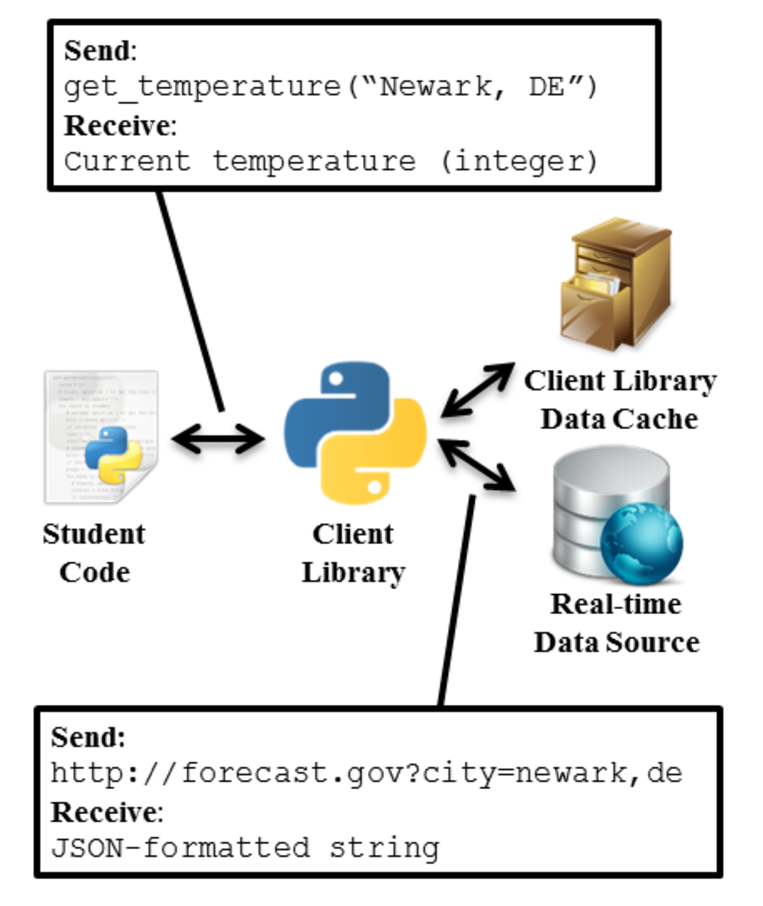
\psfig{file=images/rtw-client-library.eps, width=\linewidth}
			%\includegraphics[width=0.48\textwidth]{"images/rtw-client-library"}
    \end{center}
    \vspace{-\bigskipamount}
    \caption{RealTimeWeb Client Library Architecture}
    \label{fig-cla}
\end{wrapfigure}

Our High Volume libraries often work by providing sampled versions of the data internally, so that students can work with faster, representative subsets.
Then, when they are ready for full deployment, they can switch to a ``full production'' mode -- trading speed for quality. 
Most of the work in developing these libraries is organizing the sampled data to load into memory and get processed as quickly and naturally as possible.

An alternative scheme for distributed High Volume libraries uses a more traditional caching strategy -- assuming that the data source is largely static, requests are cached locally.
This caching is typically done using a simple key-value store on the local filesystem.
Limits can be set on the size or lifespan of the data in the cache, allowing the system to update itself according to the velocity of the external data service.
Using open-source REST API generating tools such as Eve~\cite{Eve}, existing high volume datasets can be quickly transformed into distributed datasets, alleviating the issues of data storage and transmission.

\subsubsection{Semi-Automatic Library Generation}

Our client libraries are easily available through a curated, online gallery; each library is designed to be quickly adapted to instructors' specific academic desires. 
This gallery also provides a tool for rapidly prototyping new libraries based on our framework.
As an open-source project, we encourage collaborators to explore and extend the tools that we have created.

The process of connecting to online data sources is fairly uniform: performing an HTTP request to a URL returns formatted data (typically JSON or XML). 
This information must then be parsed into native data structures, and then filtered and transformed into an appropriate domain object using the language's proper construct (e.g., structs for Racket, classes for Java).
We've established a JSON-based client library specification file format that can be compiled to appropriate source code in each of the three target languages using the modern templating language Jinja2. 
This compiler can be easily extended to new languages by providing a template.
This specification format has two major components: the functions, which connect to the relevant URL endpoints, and the domain objects, that are generated from a successful HTTP request. 
This open-source tool has been used to successfully and rapidly develop a number of the existing client libraries.

\subsubsection{Contextualizing with CORGIS}

The RealTimeWeb toolchain has been deployed for several semesters in introductory Computer Science courses for majors, ranging from the first course all the way to a Data Structures level course.
These integrations ranged from small assignments to entire semester projects using the software.
So far, the focus of the evaluation has been on the motivational influence of the system.
Quantitative data was collected by surveying students attitudes using well-established motivational frameworks and instruments, and indicates that students tended to find real-time data engaging~\cite{realtimeweb}.
In some courses, qualitative data was gathered through small group interviews, where students attribute increased engagement with the authentic, real-world connection offered by real-time data.
Similar results have been found from its integration in the Computational Thinking course -- students cite working with the realistic data as a key factor in engaging with course materials.

\begin{wrapfigure}{R}{0.5\textwidth}
		\begin{center}
				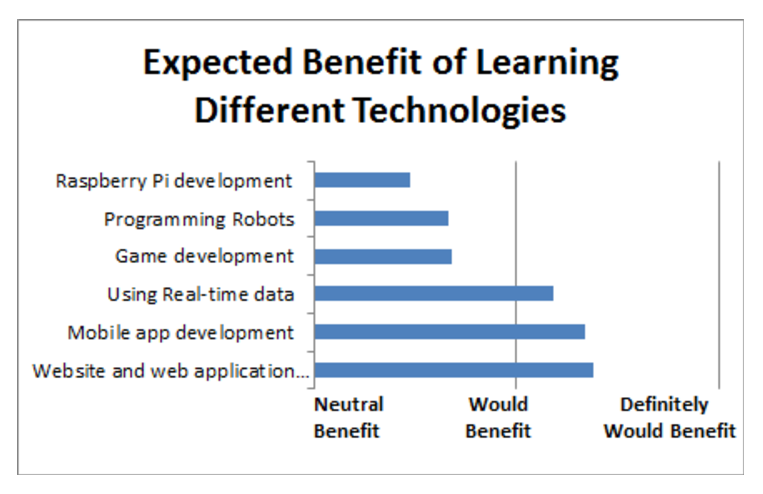
\psfig{file=images/expected-benefit.eps, width=\linewidth}
		\end{center}
		\caption{Students' Perceptions of the Benefit of Working with Learning Different Technologies}
		\label{fig-expected-benefit}
\end{wrapfigure}

\subsubsection{Limitations of CORGIS}

Although CORGIS has more or less successfully solved the problem of integrating high velocity data, and has started supporting high volume data, further work is required to solve the high variety data problem.
Furthermore, there is no principled strategy for pedagogically integrating these tools into a classroom -- instructors tend to choose data streams based on their own situational interest, rather than through a deep understanding of the affordances and limitations of the dataset.
Further work is required both on the technical and philosophical side in order to support these processes.

\subsection{Kennel}

In this section of the paper, I introduce my new online programming environment named Kennel.
The goal of Kennel is to be a beginner-friendly programming environment that scaffolds the learner into a more mature environment while supporting a number of theory-driven, pedagogical objectives.
Internally, Kennel uses a modified version of the open-source Blockly library to provide a block editor, a modified version of the open-source Skulpt library to execute python code, and an unmodified version of the open-source CodeMirror library to provide a text editor.
The system promotes the learning transfer process by supporting Mutual Language Transformation between Blockly and Python -- at any time, code can be transferred back-and-forth between the block editor and the text editor.
This transfer is highly optimized so that there is no usability delay in observing the differences between blocks and text.
Additionally, Python expressions and code blocks can be inlined inside of the Blockly program in order to provide more piece-meal integrations.

The Skulpt execution environment resides entirely within the users' browser, so there is no reliance on an external server to compile and run students' code.
This system also includes a built-in, client-side Property Explorer to support program and data visualization.
This execution environment supports a large number of native Python libraries, including custom ones developed for Big Data analysis.
The long-term goal of this project is to support a useful set of rich libraries so that sophisticated applications can be developed -- going beyond traditional console-based problems.
In this sense, the project is similar to other Skulpt-based environments such as Pythy and CodeSkulptor.
However, Kennel seeks to maintain 100\% compatibility with existing Python APIs so that all code written is authentic.

\begin{wrapfigure}{R}{0.5\textwidth}
\label{fig-blockly-custom}
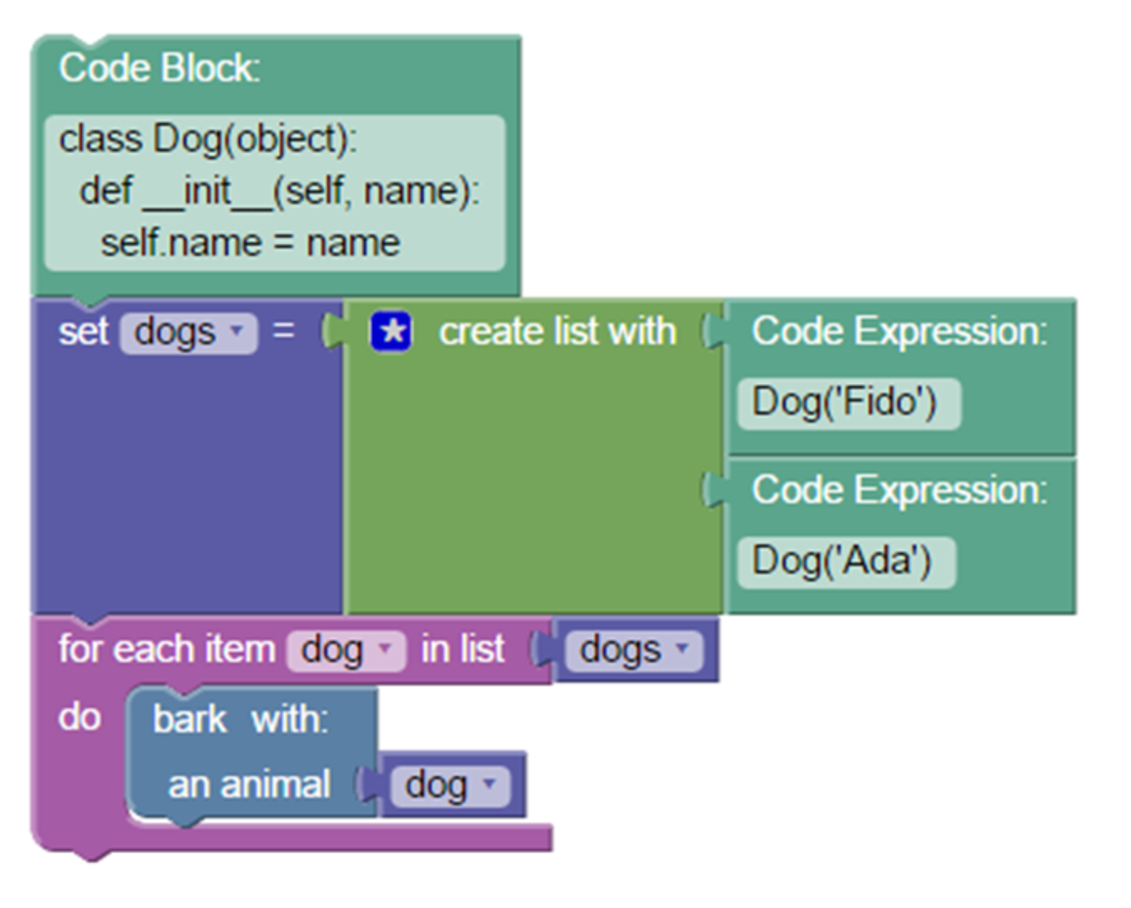
\psfig{file=images/blockly-custom.eps, width=\linewidth}
\caption{Code Block, Code Expression, and user-defined Function blocks can be used to write inline Python code}
\end{wrapfigure}

Kennel is not just a code-authoring environment but also a system for guided practice.
Instructors can create problems with interactive feedback.
As students complete and struggle with milestones within the problem, they can be given just-in-time feedback, support, and encouragement.
As they complete problems, this data can be reported to an interested central location, suitable for grading and course completion information.
The system also tracks a number of events and user interactions for fine-grained analysis.

\subsubsection{Mutual Language Translation}

Work by Weintrop on the transition from Snap to Python offers a number of ways to mediate the transfer through programming tools. 
One of the largest findings is that being able to write inline code inside a Block-based language is extremely helpful to students' learning \cite{Weintrop}.
Figure \ref{fig-blockly-custom} demonstrates how Blockly can support arbitrary code execution through the Code Block, Code Expression, and user-defined Function blocks.
This idea can be pushed further to allow students to convert their block code to textual form and then translate the textual form back to blocks.
This approach, Mutual Language Translation, is also being explored by Matsuzawa\cite{Matsuzawa} to support the transition from a desktop, block-based programming language to Java in an introductory programming class. 
Although our core approaches are similar, there are major differences.
First, translating a dynamically-typed language is a non-trivial improvement over translating a statically-typed language -- in fact, the former is technically impossible to do with 100\% accuracy, and requires a number of novel solutions in order to achieve a reasonable measure of success.
Second, my version is browser-based version, rather than relying on client-side tools, greatly enhancing the portability and providing more sophisticated student tracking.

Figure \ref{fig-mlt-overview} gives an overview of the flow of code in the environment, and figures \ref{fig-example-blockly} and \ref{fig-example-python} demonstrate the near-equivalency of the output of the two code editors.
Blockly outputs valid python source code, which can be passed into Skulpt in order to retrieve a JSON representation of the Abstract Syntax Tree.
Alternatively, the Python source of the Skulpt program can be edited directly by the user. 
Either way, this AST is parsed using our Py2Block library in order to generate an XML representation that Blockly can transform into its blocks.

Blockly already supports compilation of its blocks to Python, JavaScript, and Dart.
However, this multiple language support comes at a cost of reduced isomorphism - each language has different syntax for their common operations, and it is impossible to create a fully-featured block language with a one-to-one mapping between them.
For example, JavaScript has no support for parallel assignment, a commonly-used feature in Python, while Python does not have increment or decrement operators.

Instead of trying to satisfy multiple languages, we have dropped support for JavaScript in favor of a more full-featured mapping to Python.
Most of the changes are minor details that introduce pythonic syntax details: functions blocks are labeled ``define'', assignment blocks have an ``='' operator, the ``add item to list'' block is renamed to ``append''.
New language features are now also available -- Blockly has been extended to include support for creating and retrieving dictionaries, a crucial data structure in Python.
Some behavior of Blockly has been modified: for instance, the original code creation uses the \texttt{global} keyword within closures in order to prevent beginners from having unexpected behavior with aliased global properties -- however, this introduces additional complexity and may not be useful in a introductory context, where beginners should encounter useful struggles when they attempt to reuse global variables in a local scope.

\subsubsection{Big Data Science}

\begin{wrapfigure}{R}{0.5\textwidth}
\label{fig-mlt-overview}
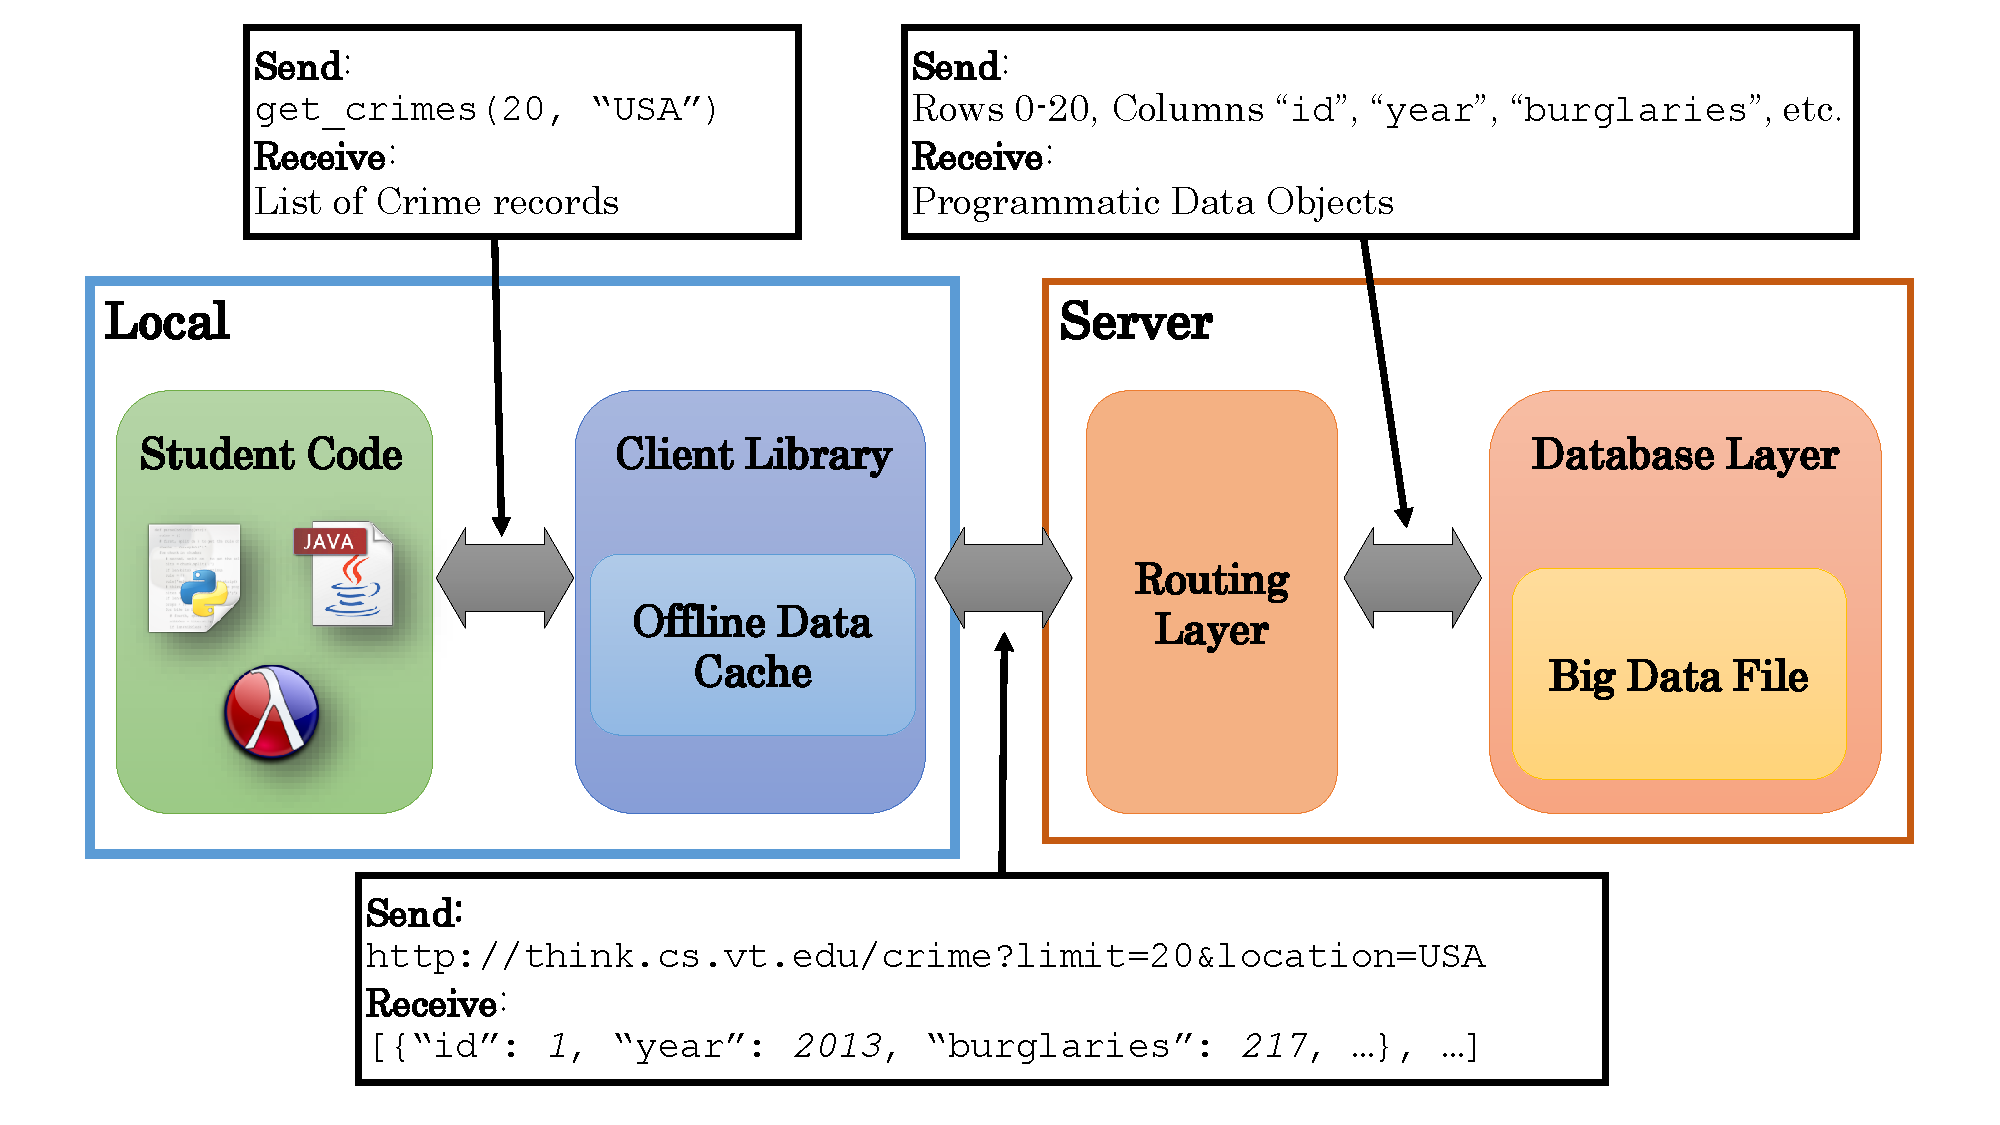
\psfig{file=images/graphics.ps, width=\linewidth}
\caption{The flow of code in the Mutual Language Translation system}
\end{wrapfigure}

In accordance with our motivational theory, we seek to move past interest-based programming into broadly useful programming contexts.
To that end, we use Data Science as an authentic context for teaching introductory computing.
As previously mentioned, Skulpt supports a number of Python APIs, and it can also be extended with any existing pure-python libraries or JavaScript libraries that use the Skulpt API.
We use a fork of Skulpt with partially equivalent implementations for the popular MatPlotlib library~\cite{SkulptMatPlotLib} and also extended it with our own implementation of the CORGIS project.
The Waywaard MatPlotLib API provides a ``plot(list)'' function to create simple line plots.
By basing everything around the MatPlotLib API, students can seamlessly shift to a serious programming environment without loss of code or productivity. 

The CORGIS (Collection of Real-time, Giant, Interesting Datasets) project strives to make it trivial to bring Big Data into introductory programming courses through carefully scaffolded libraries -- including rapidly changing high velocity data (e.g., weather, stocks) or massive high volume datasets (e.g., census and crime report data).
These libraries are pure python, and are rapidly integrated into Skulpt and exposed through the block editor, as seen in figure \ref{fig-example-blockly}.
Data returned from their interface is extremely simple -- usually either primitive (numbers and text) or simply structured (heterogenous dictionaries and homogenous lists), ensuring that students can begin working with Big Data blocks at the earliest possible point in the course.

During the course, students take advantage of the internal caching mechanism of the CORGIS libraries to work on recorded data.
This simplifies the debugging process since programs perform predictably and are no longer dependent on external data services.
When students are ready to run their programs against live data, they can move offline to a traditional programming environment and run in regular production.
This caching mechanism also benefits from an assessment view - a students program can be checked for robustness by invisibly changing the values returned by the big data functions.

\begin{figure*}[ht]
\centering
\begin{minipage}[b]{.75\linewidth}
\caption{Blockly Code}
\label{fig-example-blockly}
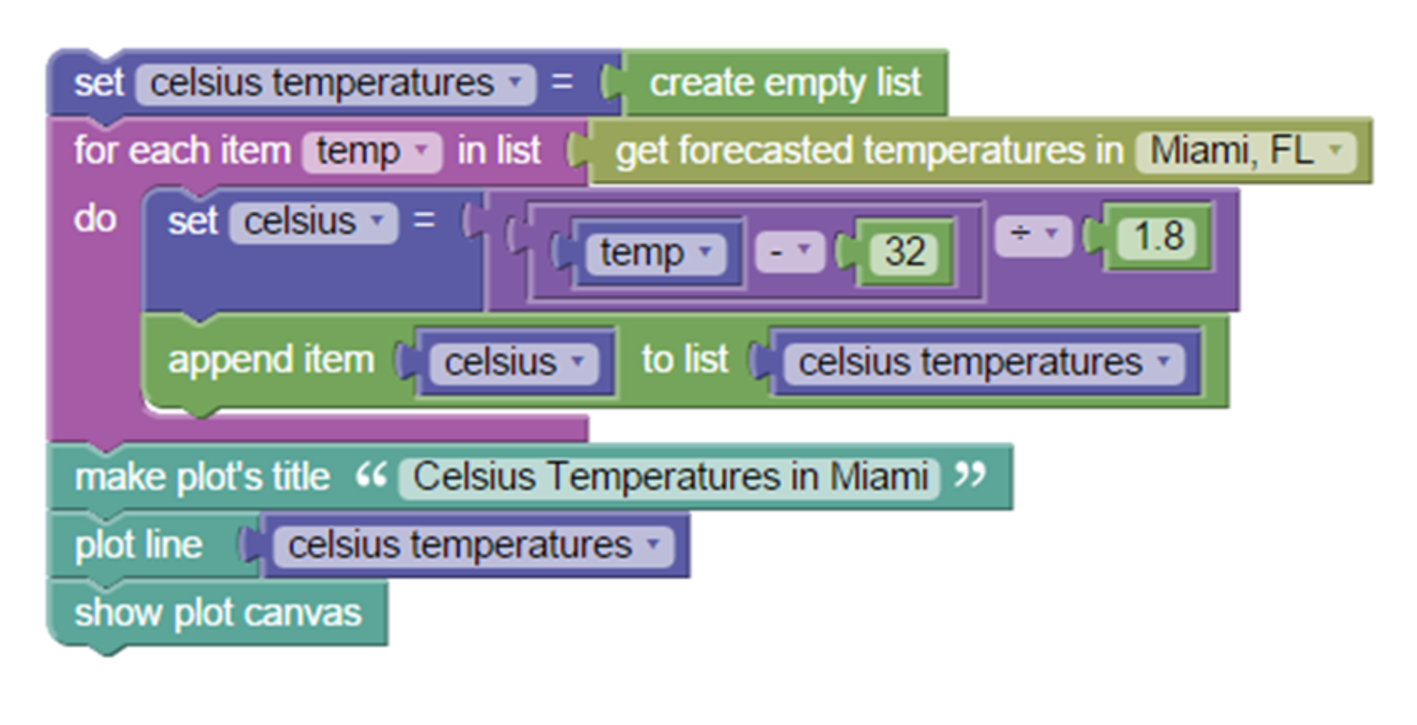
\psfig{file=images/blockly-example.eps, width=\linewidth}
\end{minipage}

\smallskip

\begin{minipage}[b]{.75\linewidth}
\caption{Python Code}
\label{fig-example-python}
\begin{python}
import weather
import matplotlib.pyplot as plt

celsius_temperatures = []
for t in weather.get_temperatures("Miami, FL"):
	celsius = (t - 32) / 1.8
	celsius_temperatures.append(celsius)
plt.title("Celsius Temperatures in Miami")
plt.plot(celsius_temperatures)
plt.show()
\end{python}
\end{minipage}
\end{figure*}


Eventually, more sophisticated visualizations will be required.
Users are often highly motivated to create user interfaces to control their software interactively.
By supporting a GUI library like TKinter or PyQT, students could construct an entire python program in the browser, and then immediately share their work with friends, families, and potentially even colleagues.
This overcomes a limitation of traditional python development - python code can only be run in a Python interpreter with the appropriate libraries, and most end-users do not have such software already installed.
Once relevant libraries are added to our Skulpt fork, students can create and share sophisticated programming projects seamlessly.

\subsubsection{Guided Problems}

A limitation of programming environments like Snap! is that they are not meant to be pedagogically interactive - students completing an assignment in the system are not guided to success.
Instead, they are given a blank canvas and expected to work towards some externally defined goal, only knowing they are complete according to some external measurement (e.g., a problem description given by an instructor).
Although this is tremendously useful for free-form constructivist and discovery learning experiences, they limit the system's ability to guide students that are just starting out.
To provide these more scaffolded learning experiences, Kennel includes a mechanism for problems.

A problem in Kennel includes a rich text description and instructor-provided logic.
This logic is specified as a prioritized mapping of predicates to messages -- the student's code and the output of their program's execution are passed to the predicates and matched against their ordered.
When a predicate is triggered, the student is offered the corresponding message -- a suggestion or motivational remark, depending on what the instructor has made available.
A common example is a predicate that checks whether the students used iteration (e.g., a \texttt{foreach} loop) within their code, and then warns the student that iteration is required for that problem.
In a large class size, this simplistic but automated feedback is tremendously useful.
However, the API is currently very limited, resulting in a large investment by the problem designer in creating new materials and hints.

\subsubsection{Persistence and Event Tracking}

In my pilot of Kennel, the system is embedded within an online, interactive textbook based off the popular Runestone platform. % Cite runestone
All work completed by the student is reported to the system in order to assign course credit.
Additionally, in-progress development is persisted on the server using a fault-tolerant caching mechanism, described in Figure \ref{ft-cm}.
\begin{figure}
\begin{enumerate}
  \item User triggers a change \textit{Or} Client reloads page, and an entry is found in the LocalStorage.
	\item Change is stored in LocalStorage.
	\item Change is sent to server.
  \item Server successfully stores change \textit{Or} Fails to store the change.
	\item Upon receipt of successful change, the Client clears entry in LocalStorage \textit{Or} It never recieves the receipt and instead keeps the entry until a page reload.
\end{enumerate}
\caption{Fault-Tolerant Caching Mechanism}
\label{ft-cm}
\end{figure}
Finally, all student interactions with the systems' user interface are tracked for logging purposes.
This includes students program edits, down to nearly the key-stroke level.
These can be used in order to build up a complete representation of the students code as they develop, furthering the analysis of student programs for common patterns of mistakes.

    \section{Proposed Technical Work}

To help support testing my hypotheses, a number of new pieces of technology and instruction will need to be created.

\subsection{Sophisticated Data Exploration}

Understanding the structure, meaning, and values of data can be a difficult problem for introductory students.
Using Data Science as the introductory context puts an increased emphasis on data structures and algorithms, making this content more critical for the learner.
Currently, there are not many tools available through Kennel to scaffold students.

The Property Explorer is probably the current greatest tool available to students for understanding program state.
However, field trials with it show that most students do not take advantage of the tool, with few reported events in the systems' tracker.
The usability of the property explorer, and its connection to the concept of Program State, must be elucidated to the student more clearly.

More tools are also desirable for engaging learners.
A number of graphical representations are used throughout the Computational Thinking course in order to visualize topics such as Abstraction and program flow.
For instance, students build Data Map Diagrams as seen in Figure \ref{data-maps-weather}, intended to help them navigate complex data structures.
The system can be extended to create simplified graphical visualizations of the students code and the data model in order to connect to these other course topics.

Currently, the implementation of MatPlotLib and other APIs is very minimal -- eventually, complete support for their functionality is needed.
There are other novel additions that can be introduced too -- for example, recent work by \cite{pixly} integrates media computation into Blockly environments.
By integrating such material into Kennel, we can provide students a comparative point between the different introductory programming contexts, in order to meaningfully evaluate the affordances of the different approaches.
Crucially, care must be taken to keep Kennel as a pure Python programming environment, without introducing cumbersome non-standard 3rd party libraries as occurs in CodeSkulptor~\cite{code-skulptor}.
As all of these materials extend the functionality of Kennel is new and innovating ways, but this material is less valuable if it reduces the authenticity and transferability of the learning experience.

\subsection{Complete Mutual Language Translation}

One of the biggest features of Kennel is the Mutual Language Translation, and this is where I expect a large amount of technical work will need to be done.
Indeed, there are a number of unsupported Python language features: classes are probably the biggest offender, but there are many other desirable features missing such as list unpacking, tuples, and sets.
These must be introduced to the system gradually and gracefully so that a beginner is neither overwhelmed nor distracted.
In some cases, incorporating these changes will require massive internal changes to Blockly's ability to represent concepts.

An ideal interface should offer a complete isomorphic mapping to Python - however, there are a number of complications to resolve before that can occur.
For instance, Python uses square brackets for both list indexing and dictionary access.
There is a strong desire to differentiate between these distinctive types of access, visible in the block view as two distinct kinds of blocks (``get ith element of list'' vs. ``get key from dict'' blocks).
Although some indexes are syntaxically unambiguous -- e.g., a string literal used as an index *cannot* be for a list -- there are many that are impossible to determine at compile-time using traditional static analysis.
This is largely because Python is a dynamic language -- the parser has no idea what type a variable has, so it is impossible to tell if a given variable is a dictionary or a list.
Instead, dynamic analysis needs to be combined with abstract interpretation techniques, such as those used in PySonar~\cite{PySonar}.
Typically these systems suffer from state explosion due to the large number of metaprogramming techniques usable in a python programmer - however, they are uniquely suitable for an educational environment due to the reduced subset of Python needed in practice by beginners.

A less technical and more user-oriented question is how many language details should be exposed, and what rate.
A rarely used feature of ``for'' loops in Python is to contain an ``else'' clause that is executed upon successful completion of the loop (that is, when it is not prematurely escaped using a ``break'' statement).
This advanced language feature is meant to draw special attention to connected actions that must be performed after the iteration is completed.
If an ``else'' clause were made available to beginners first trying to grapple with iteration, it is likely they would confuse the concept with the conditional ``else'' clause used in ``if'' statements.
Cognitive Load Theory can be a harsh mistress for beginners, and the user interface needs to avoid exposing unnecessary details where possible.
It can be very difficult to recognize when the learner is ready to understand parallel assignment, and therefore able to specify multiple variables on the left side of an assignment block.
This is actually an advantage of traditional text-based environments, since they hide all advanced features by their very nature.

However, there are techniques that can be applied to infer the types of most variables.
Simple dynamic analysis can be used to infer the type of a property over the course of the programs execution.
Certain restrictions can be made towards beginner's codes that, while draconian to an experienced developer, are reasonable for someone starting out.
For instance, we might require that a beginner only allow a property to take on a single type, issuing an error if they do not.
There are other edge cases that must be dealt with in a principled fashion.
It is impossible to predict the type output of ``eval'', for instance -- but fortunately, ``eval'' is bad practice in general and should also be forbidden to beginners.

\subsection{Meaningful Program Analysis}

In a classroom of many students and minimal instructors, it is a challenge to keep students successful.
Most students lack the programming knowledge to identify their own errors, let alone diagnose and fix them.
Although 1-1 human tutoring is ideal for learners, there are simply not enough staff resources.
For some kinds of problems, the system can support the student.

WebCAT\cite{webcat} is a well-known tool for solving this problem -- it uses style checks and unit testing to identify mistakes and make suggestions to the student.
There are other tests that can be used too.
A limitation of systems like WebCAT is that they often depend on a specific code shape: usually, they operate over explicit function contracts.
For example, students might be assigned to write a \texttt{sum} function which consumes an array of integers and returns a single value representing their summation -- students that do not match this contract can be guided.

Kennel already provides a limited API for providing such support, but it is extremely ad-hoc.
I propose a richer API for analyzing student code and tracking deficiencies.
Figure \ref{fig-example-analysis} provides a potential mock-up of this system.
The instructor implements a function that consumes some information about the students' code, and then returns feedback for the student and the system.
This API could additionally query for prior students mistakes, in order to provide more contextualized assistance -- if a student consistently iterated over an empty list, for instance, this could be representative of a greater understanding rather than a typo, and small hints would be less useful to their long-term learning than instructor intervention.

\begin{figure*}[ht]
\definecolor{mymauve}{rgb}{0.58,0,0.82}
\lstset{stringstyle=\color{mymauve}}
\lstset{
   language=JavaScript,
   backgroundcolor=\color{lightgray},
   extendedchars=true,
   basicstyle=\footnotesize\ttfamily,
   showstringspaces=false,
   showspaces=false,
   numbers=left,
   numberstyle=\footnotesize,
   numbersep=9pt,
   tabsize=2,
   breaklines=true,
   showtabs=false,
   captionpos=b
}
\begin{lstlisting}[columns=fullflexible]
function check(code, ast, variables) {
  // Did the student use too many or too few loops?
	if (ast.getIterations() != 1) {
	  // Give them a helpful message, and identify that they
		// made an iteration-related mistake.
	  return {'message': 'You are not iterating the right number of times!',
		        'mistakes': ['iteration']};
	}
	// Get the proper loop
	var iteration = ast.getIterations()[0];
	// Get the list we looped over
	var iteration_list= iteration.getList();
	// Check the state changes of the list over the program's life
	var list_states = variables[iteration_list];
	// Are they iterating over an empty list?
	if (isAlwaysEmptyList(list_states)) {
		return {'message': 'You are iterating over an empty list!',
		        'mistakes': ['iteration', 'program state']};
	}
	// Are they appending to the iterating list?
	if (changesAfterInitialization(list_states)) {
	  return {'message': 'You are changing at list as you iterate over it.',
						'mistakes': ['append']}
	}
	...
}
\end{lstlisting}
\caption{Analysis API Mock-up}
\label{fig-example-analysis}
\end{figure*}

In addition to the static program analysis, dynamic program analysis can also be used.
The custom libraries actually provide a useful mechanism for conducting behind-the-scenes unit testing.
A student submits code such as in \ref{fig-example-blockly}.
This code depends on a special CORGIS library that returns weather data, in particularly retrieving the weather for a specific city.
When the students code is evaluated by the system, this libraries functions can be repeatedly rerun to return different data -- substituting ``Blacksburg, VA'' as the argument, and ensuring that the students code returns the proper value.
This approach avoids more easily-abused output-checking, which students can fool by printing literal values as opposed to computed values.

Data Flow Testing can also be critically useful in evaluating students' code.
By observing the value changes that a property takes over time, common errors can be revealed.
The non-existence of an expected value can also be instrumentative.
A common beginner mistake is to not assign the output of an expression to a property -- either discarding the value entirely, or printing it instead.
A system could diagnose a missing value from the overall flow and suggest the user investigate the program state over time, or even revisit the lesson on the subject.

\subsection{Student Tracking and Reporting}

In order to scale the learning experience, instructors and course staff need to have access to a wealth of information about students.
No matter how involved and committed the staff is, they will be out-of-touch with some of these students.
This information involves motivation (do the students feel that they can succeed?), engagement (has the student been attending class?), ability (does the student understand iteration?), demographic (what major is this student?), and other dimensions of learning.
I propose creating a system, tied strongly to Kennel, to track students across as many dimensions as is useful and practical, in order to provide just-in-time reports for staff and the learners.

Much of this information needs to be made available quickly -- course staff cannot spare much time getting grounded on the history of the student.
During office hours, multiple students might show up at once.
A teaching assistant would wish to know who needs the most help, and what challenges individual students have already had.
For instance, a student might have already met with other TAs many times, indicating that they are struggling a lot in this course.
Although this is information that can be obvious with only a few minutes of interaction with the students, there is much time and energy wasted.

Course staff often meet regularly to assess the ``problem students'' and ``success students''.
The staff often make valuable estimations of their learners abilities and motivation, both in general and specifically.
This data could be captured by the system and used to drive the feedback being made available.
It can also be tremendously useful in course retrospectives.

The system can also assist in making interventions to support students.
Although hints and suggestions are obvious, there are other mechanisms too.
Students can be reminded of course goals that they have established (appealing to their long-term objectives).
Automated, self-regulatory suggestions can be sent to the learners when they have not engaged with the materials in a while, suggesting that they try out a problem for a while to see if they can make some progress (or at least identify their misconception) or move onto lateral material so they can make headway elsewhere.
Staff can be notified of a particularly struggling student, in order to encourage them to reach out with suggestions or encouragement.
Finally, situational interest could be appealed to with motivational content such as inspiring quotes, amusing images, or other rewards.

\subsection{More Libraries}

The CORGIS project depends on having an extensive and varied collection of datasets. 
Students should be able to find a dataset that appeals to their personal interests but provides a sound learning experience.
Making this experience relatively uniform is challenging, but makes providing support much easier -- a necessary element in a scaled classroom.

The same data source can be expressed in many ways, representing different levels of abstraction and different affordances.
Consider the data map in figure \ref{data-maps-weather}, representing potential structures for weather data collected about cities around the world.
Although maps A and B contain the exact same data, they are structured very differently -- a list of cities vs. a dictionary of cities.
For an experienced programmer, these differences are minor details that have implications for runtime performance: looking up a city's temperature is slower and more complicated in structure A (requring iteration and decision) than it is in B (requiring only dictionary access).
Although the differences in code are minor to an expert, they require fundamentally different areas of knowledge for a beginner.
Map C represents an entirely different level of abstraction, where weather is only represented as a numeric, without information about cities.
The number of questions that can be answered using this data is greatly reduced -- statistics about cities in general, rather than comparisons against specific cities.
And of course, the nature and schema of the data itself affects the types of questions that can be asked -- it makes sense to find the average of a list of temperatures, but not the sum.
A key part of my research will be explicitly identifies trade-offs and affordances of different structures and abstractions of data.

\begin{figure}
\begin{center}
\tikzset{
    bnode/.style = {   
        align=center, draw,
        rectangle split, rectangle split horizontal,
				rectangle split draw splits=false
    }
}
\begin{minipage}{.4\textwidth}
\begin{tikzpicture}
    \node[align=center, draw] (root)
		  {List of}
		;
		\node[bnode, below=of root,rectangle split parts=3]
       (middle)
       {	\nodepart{one}
					Dictionary of:
					\nodepart{two}
          ``city'' ,
					\nodepart{three}
					``temperature''
					};
		
    \draw (root) -- (middle);
    \draw (middle.two south) -- +(0, -1) node[draw, anchor=north](q) {string};
    \draw (middle.three south) -- +(0, -1) node[draw, anchor=north](q) {integer};
		%  +(0,-1) 
\end{tikzpicture}
\begin{center}
(A) List of Weathers
\end{center}
\end{minipage}
\begin{minipage}{.4\textwidth}
\tikzset{
    bnode/.style = {   
        align=center, draw,
        rectangle split, rectangle split horizontal,
				rectangle split draw splits=false, rectangle split parts=4
    }
}
\begin{tikzpicture}
		\node[bnode]
       (root)
       {	\nodepart{one}
					Dictionary of:
					\nodepart{two}
          ``blacksburg'' ,
					\nodepart{three}
					``newark'',
					\nodepart{four}
					``venice''
					};
		
    \draw (root.two south) -- +(0, -1) node[draw, anchor=north](q) {integer};
    \draw (root.three south) -- +(0, -1) node[draw, anchor=north](q) {integer};
		\draw (root.four south) -- +(0, -1) node[draw, anchor=north](q) {integer};
		%  +(0,-1) 
\end{tikzpicture}
\begin{center}
(B) Dictionary of Weathers
\end{center}
\end{minipage}


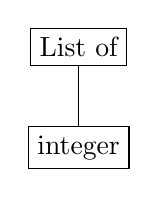
\begin{tikzpicture}
		\node[align=center, draw] (root)
		  {List of}
		;
		
    \draw (root) -- +(0, -1) node[draw, anchor=north](q) {integer};
		%  +(0,-1) 
\end{tikzpicture}
\begin{center}
(C) List of Temperatures
\end{center}

\end{center}
\caption{Weather Data Maps}
\label{data-maps-weather}
\end{figure}

Finding data sources can be a challenging task.
A component of my research plan is to publish best practices and techniques for finding, organizing, and exposing datasets.
The CORGIS collection already contains three dozen libraries, covering areas as diverse as international studies, nutrition, and social media platforms.
Some datasets were chosen because they were low-hanging fruit -- extensively documented, freely available, and well-supported. 
However, other datasets were driven by students' needs; in the two semesters that the course has been offered, two dozen new datasets have been created on demand.
The rapid turn-around time required has given new insight into the process of data mangling, although I am still exploring methods.
A massive part of my proposed work is to solidify and publish these techniques into a full paper.

    \section{Planned Intervention}

With the development of the new technology, interventions will be staged through Virginia Tech's new ``Introduction to Computational Thinking'' course, created to help fulfill the university's new General Education Requirements~\cite{vt-vision}. 
This course has already been run for two semesters, deeply incorporating much of my existing research work.
The course is taught and developed primarily by Dr. Dennis Kafura, although I have also been involved as associate instructor, managing course materials, server and technology administration, and assisting with in-class teaching.
However, now that the course is more solidly defined, my role is shifting into a more observational function in order to drive my dissertation work.
As a research endeavor, the course is heavily instrumented to provide data on its novel pedagogies and technologies.
Although there are confounding factors to working with such a heavily experimental course, it presents a unique testbed for materials and is an excellent source for mining research results.

\subsection{The Learners}

In the first offering of the course, 25 students enrolled in the course, and 20 students finished the coursework.
In the second offering, 40 students initially enrolled and 35 successfully passed the course.
Figure \ref{data-demographics} indicates the relevant demographic data collected through surveys.
Largely, the students represent the population at Virginia Tech, albeit with some disproportion towards certain majors than others.
It is worth pointing out the excellent gender diversity within the class.

\begin{figure*}
\begin{minipage}{\linewidth}
\centering
	\begin{tabular}{c|c|c}
	  \multicolumn{3}{c}{Gender}\\\hline
		& Fall 2014 & Spring 2015 \\\hline
		Female & 6 & 21 \\
		Male & 13 & 18 \\
	\end{tabular}
\centering
	\begin{tabular}{c|c|c}
	  \multicolumn{3}{c}{Prior Programming Experience}\\\hline
		& Fall 2014 & Spring 2015 \\\hline
		Yes & 10 & 7 \\
		No & 10 & 32 \\
	\end{tabular}
\centering
	\begin{tabular}{c|c|c}
		\multicolumn{3}{c}{Year}\\\hline
		& Fall 2014 & Spring 2015 \\\hline
		Freshman & 2 & 5 \\
		Sophomore & 7 & 11 \\
		Junior & 6 & 11 \\
		Senior & 5 & 10 \\
		Unknown & 0 & 2 \\
	\end{tabular}
\centering	
	\begin{tabular}{c|c|c}
	  \multicolumn{3}{c}{Colleges}\\\hline
		& Fall 2014 & Spring 2015 \\\hline
		Engineering & 2 & 2 \\
		Agriculture & 0 & 1 \\
		Sciences & 7 & 5 \\
		Liberal Arts & 9 & 23 \\
		Architecture & 1 & 7 \\
		Natural Resources & 0 & 0 \\
	\end{tabular}
\caption{Demographic Data of Computational Thinking Students}
\label{data-demographics}
\end{minipage}
\end{figure*}


\subsection{The Content}

Virginia Tech defines four learning objectives for computational thinking. Students are required to:
\begin{enumerate}
	\item Apply computational methods to model and analyze complex or large scale phenomena.
	\item Formulate problems and find solutions using computational or quantitative thinking in their field of study.
	\item Give examples of the application to, and discuss the significance of, computational thinking in at least two different knowledge domains. 
	\item Evaluate the social and political impact of computing and information technologies 
\end{enumerate}

This content is mapped roughly into four instructional units on Computational Modelling, Algorithms, Data Intensive Inquiry, and Social Impacts. The lattermost unit is threaded throughout the course, while the first three are roughly sequential. Figure \ref{course-outline} gives a high-level overview of the content of this course.

\begin{figure*}
\begin{tabularx}{\textwidth}{ |l|X| }
\hline
Topic (Length) &	Description \\\hline
Computational Modeling \newline\newline
 (2 weeks) & Model-based investigation of how complex global behavior arises from the interaction of many “agents”, each operating according to local rules. Students use case-based reasoning and encounter basic computation constructs in a highly supportive simulation environment. \\\hline
Fundamentals of Algorithms \newline (4 weeks) & Study of the basic constructs of programming logic (sequence, decisions, and iteration) and program organization (procedures). A block-based programming language is used to avoid syntactic details. Students can see how these constructs are expressed in Python. \\\hline
Data-intensive Inquiry \newline (7 weeks) & Project-based exploration of complex phenomena by algorithmically manipulating large-scale data from real-world sources. Students construct algorithms in Python using a supportive framework for accessing the data. \\\hline
Social Impacts \newline (2 weeks) & Explore and discuss contemporary societal issues involving computing and information technology. \\\hline
\end{tabularx}
\caption{High-Level Course Overview}
\label{course-outline}
\end{figure*}


\subsection{The Course}

The course uses a considerable amount of modern pedagogical techniques, many of which represent ongoing research questions.
Perhaps the most influential technique is the organization of students into cohorts.
Near the beginning of the semester, students are put into groups of 5-6, balancing based on year and gender where possible, and avoiding putting similar majors into the same group.
These cohorts primarily function as a support structure that students can rely on to get help and encouragement.
Although cohorts work together on many smaller in-class assignments, every student is ultimately responsible for their own work -- the final project, for instance, is individual to each student.

Class time is split between presentation (typically stand-up lecture) and participation (typically computer-based work or cohort discussion) using an Active Learning style whereever possible.
Earlier questions in the course often have students completing questions on paper or doing more kinetic exercises.
Later questions rely on the automated Kennel questions, until the students reach the open-ended project work.

Work in the class is considered to be under a mastery style -- deadlines are enforced only in so far as they motivate students to complete assignments, not in order to punish.
Students are free to work on the material as long as they need.
A recurring message within the course is that ``failing is okay, as long as you keep trying''.

\subsection{The Research Protocol}

The Computational Thinking course is deeply integrated into my research technology -- the middle section of the course uses Kennel as the programming environment, and the last section of the course uses CORGIS to manage the students' projects.
Every semester, students will be surveyed at the start, middle, and end of the course in order to collect relevant data.
Their interactions with the technological systems will be tracked at a fine-grained level, as will be their final projects.
This data can be compared across semesters as it accumulates in order to hit instructor-set goals.
Along the way, important questions related to secondary research goals can also be answered -- how to design CORGIS libraries, the affordances of Data Science as an educational tool, and the pedagogical strategies for using Kennel.

\subsection{Measuring Success}

There are three primary dimensions used in measuring the success of my proposed work: students' motivation, students' ability, and the courses' scalability.
Different instruments and sources will be used to track and measure the impact of the various research efforts.
Ultimately, gains are expected as materials are refined, ideally achieving some established performance objectives.

\subsubsection{Motivation}
Motivation in the course will be primarily assessed through self-reported surveys based heavily on the MUSIC Model of Academic Motivation Inventory (MMAMI).
Students will be non-anonymously surveyed using the complete instrument at key points in the semester, and regularly surveyed using a miniaturized version throughout the semester.
These miniaturized versions will be used as follow-ups to specific course exercises in order to determine more finely-grained answers about where students found motivation.
Additionally, targeted qualitative data will be gathered in order to refine this quantitative data.

This motivational data will be combined with evidence of engagement with the course across several different dimensions. Therefore, the complete list of motivational sources is:
\begin{description}
	\item[Attendance:] Did the students regularly attend class?
	\item[Retention:] Did the students complete the course with a passing grade?
	\item[Coursework:] Did the students regularly complete coursework and homework on time?
	\item[Struggle:] Did the students continue with materials even after setbacks?
	\item[Continuation:] Do students intend to follow-up the course with further courses and learning experiences in Computational Thinking?
	\item[Observations:] Did the course staff report students as being motivated, according to their own observations?
	\item[Self-report:] Did the students report themselves as being motivated, according to MMAMI and other surveys?
\end{description}

\subsubsection{Ability}
There are several high-level course concepts that students are expected to gain some level of mastery in during this course.
There are also lower-level skills that students should gain some familiarity with.
Although this is not a programming course, per se, success will be partially measured based on students success with the computational elements of the material.
However, the success of the course will be foremost evaluated on the high-level concepts, such as the role of Abstraction and Algorithms.

The most important element measuring students' ability is the final project, a performance assessment where students solve a self-guided, computationally-oriented problem that they might realistically find in their chosen profession.
Students choose their own dataset (through CORGIS), problems, and approach based on the techniques learned in the course and supported by the course staff.
Course staff are ultimately responsible for evaluating their completed project (instantiated as a codebase and a video presentation) against a rubric that measures several of the higher learning objectives.
This form of assessment is viewed as more authentic than alternatives such as a final exam or a concept inventory, given the complicated nature of measuring high-level conceptual skills such as Computational Thinking.

Smaller, low-stakes, pre- and post- assessments will also be collected during the semester for individual instructional units in order to gather data on students’ ability with specific, lower-level course content (e.g. programming concepts such as loop iteration and dictionary access).
This data will be supplemented by fine-grained, automatically-collected student solutions to coding problems in order to evaluate student progress throughout their interactions with an assignment, rather than purely summatively.
Finally, course staff will be regularly and systematically interviewed in order to identify the commonly-occurring questions and challenges that students raise.
Ultimately, this data should approach some specific measurement of success -- this specific measure will be determined shortly before the preliminary proposal based on data collected during the first two course offerings.
As a rough measure, 70\% of the students should achieve a ``high'' level of understanding of all the course concepts, and no more than 15\% of the students should achieve a ``low'' or worse level of understanding, as measured by the instructors.

\subsubsection{Scalability}
As a major stakeholder in the course, the instructors’ experience is also crucial to understanding the success of our approach.
As the course scales in size, it is both expedient and proper that an instructor have a feel for their learners.
The technology in the course must support this process wherever possible – for example, an instructor meeting with a student during office hours must immediately know the students current state in the course, both motivationally and ability-wise.
Course staff will be regularly interviewed in order to identify successes and failures of the automated tools in managing a large-scale course.
Students will also be interviewed and surveyed to assess their perception of the courses size – e.g., whether feedback came timely enough, they had the in-class support they needed to succeed, they felt satisfied with the human interactions in the course.


    \section{Work and Publication Plan}

My primary publication venues 

\begin{easylist}[itemize]
& Spring 2015
&& Second offering of CT course, collect baseline data (N=40)
&& ICER'15 Doctoral Consortium Proposal
&& Alpha version of Kennel
&& Second iteration of CORGIS libraries being used in a course
& Summer 2015
&& Preliminary Proposal
&& TOCE Journal Paper on Big Data Science Affordances
&& Beta version of Kennel
& Fall 2015
&& SIGCSE'16 Paper publicly announcing and describing Kennel, offer workshop on Kennel
&& Third offering of CT course, collect data (N= expected 40-80)
& Winter 2016
&& ITiCSE'16 Paper on program analysis of block-based python programs
& Spring 2016
&& Fourth offering of CT course, collect data (N= expected 80)
& Summer 2016
&& Development of second iteration of Kennel
&& Finalization of all major CORGIS architectures
&& TOCE Journal Paper on the design and issues of Virtual Learning Environments
& Fall 2016
&& Fifth offering of CT course, collect data (N= expected 80)
&& SIGCSE'17 Paper on affective/cognitive student tracking in Kennel
& Spring 2017
&& Sixth offering of CT course, collect data (N= expected 80)
&& ICER'17 Paper, as a summative view of my primary research questions (using CORGIS and Kennel to meaningfully motivate and guide large quantities of students to success).
&& Final Thesis Defense
\end{easylist}
    \section{Conclusion}

My research is focusing on motivating and scaffolding introductory computer science classes.
I seek to introduce new tools and approaches that can support large-scale, in-person classroom experiences while still appealing to the unique kinds of learners that approach computing in higher learning.
In this preliminary proposal, I describe the technical work and how it will be deployed and evaluated in a Computational Thinking classroom.
I anticipate that this approach to introductory computing will provide useful new techniques and tools instructors.
Adoption of the materials will vary widely, with some instructors taking the curriculum wholesale and some just using pieces of it.
However, the tools will be readily available and the experience will indicate how they can be used most effectively.
		
    
% Appendix
\newpage
		\appendix

\section{Appendix}

\subsection{Weinberg Computational Thinking Research Taxonomy}\label{app:weinberg-taxonomy}
    
    The following taxonomy is taken from~\cite{weinberg2013} and classifies the various types of papers in the literature.
    
    \begin{description}
        \item[Curriculum Description (48\%)] Articles that explain a lesson, curriculum, activity, or course that is used to promote computational thinking or one of its domains
        \item[Program Description (7\%)] An intervention or idea that goes beyond the individual classroom level and is implemented on a larger scale � across a university, for example.
        \item[Evaluations (5\%)] The primary aim for the paper was to convey the results of a study focused on a specific program or intervention. This goes beyond the prior two sections in that they emphasize evaluation methods and findings.
        \item[Research (12\%)] Distinguished from evaluations by their focus on informing theory or contributing to the larger knowledge base rather than being focused on a single program or intervention.
        \item[Philosophy (23\%)] Papers intended to create or promote debate about computational thinking in the broad computer science or computer science education communities. Works in this category might aim to share a perspective on an issue within the field or describe how CT applies to other disciplines.
        \item[Opinion (6\%)] Similar to Philosophy, except with a more subjective perspective; they are typically not peer-reviewed.
    \end{description}
    
\subsection{Dominant Definitions of Computational Thinking}\label{app:ct-definitions}
    
    \subsubsection{AP CS Principles}
    
    \begin{description}
        \item[P1: Connecting computing] \hfill \\
        Developments in computing have far-reaching effects on society and have led to significant innovations. These 
        developments have implications for individuals, society, commercial markets, and innovation. Students in this 
        course study these effects and connections, and they learn to draw connections between different computing 
        concepts. Students are expected to: 
        \begin{itemize}
            \item Identify impacts of computing; 
            \item Describe connections between people and computing; and 
            \item Explain connections between computing concepts. 
        \end{itemize}
        
        \item[P2: Developing computational artifacts] \hfill \\
        Computing is a creative discipline in which the creation takes many forms, ranging from remixing digital music 
        and generating animations to developing websites, writing programs, and more. Students in this course engage 
        in the creative aspects of computing by designing and developing interesting computational artifacts, as well as 
        by applying computing techniques to creatively solve problems. Students are expected to: 
        \begin{itemize}
            \item Create an artifact with a practical, personal, or societal intent; 
            \item Select appropriate techniques to develop a computational artifact; and 
            \item Use appropriate algorithmic and information-management principles. 
        \end{itemize}
        
        \item[P3: Abstracting] \hfill \\
        Computational thinking requires understanding and applying abstraction at multiple levels ranging from privacy 
        in social networking applications, to logic gates and bits, to the human genome project, and more. Students in 
        this course use abstraction to develop models and simulations of natural and artificial phenomena, use them to 
        make predictions about the world, and analyze their efficacy and validity. Students are expected to: 
        \begin{itemize}
            \item Explain how data, information, or knowledge are represented for computational use; 
            \item Explain how abstractions are used in computation or modeling; 
            \item Identify abstractions; and 
            \item Describe modeling in a computational context. 
        \end{itemize}
        
        \item[P4: Analyzing problems and artifacts] \hfill \\
        The results and artifacts of computation, and the computational techniques and strategies that generate them, 
        can be understood both intrinsically for what they are as well as for what they produce. They can also be 
        analyzed and evaluated by applying aesthetic, mathematical, pragmatic, and other criteria. Students in this 
        course design and produce solutions, models, and artifacts, and they evaluate and analyze their own 
        computational work as well as the computational work that others have produced. Students are expected to: 
        \begin{itemize}
            \item Evaluate a proposed solution to a problem; 
            \item Locate and correct errors; 
            \item Explain how an artifact functions; and 
            \item Justify appropriateness and correctness. 
        \end{itemize}
        
        \item[P5: Communicating] \hfill \\
        Students in this course describe computation and the impact of technology and computation, explain and justify 
        the design and appropriateness of their computational choices, and analyze and describe both computational 
        artifacts and the results or behaviors of such artifacts. Communication includes written and oral descriptions 
        supported by graphs, visualizations, and computational analysis. Students are expected to: 
        \begin{itemize}
            \item Explain the meaning of a result in context; 
            \item Describe computation with accurate and precise language, notation, or visualizations; and 
            \item Summarize the purpose of a computational artifact. 
        \end{itemize}
        
        \item[P6: Collaborating] \hfill \\
        Innovation can occur when people work together or independently. People working collaboratively can often 
        achieve more than individuals working alone. Students in this course collaborate in a number of activities, 
        including investigation of questions using data sets and in the production of computational artifacts. Students 
        are expected to: 
        \begin{itemize}
            \item Collaborate with another student in solving a computational problem; 
            \item Collaborate with another student in producing an artifact; and 
            \item Collaborate at a large scale
        \end{itemize}
    \end{description}
    
    \subsubsection{CSTA}
    Computational thinking (CT) is a problem-solving process that includes (but is not limited to) 
    the following characteristics: 
    \begin{enumerate}
        \item Formulating problems in a way that enables us to use a computer and other tools to help solve them.
        \item Logically organizing and analyzing data
        \item Representing data through abstractions such as models and simulations
        \item Automating solutions through algorithmic thinking (a series of ordered steps)
        \item Identifying, analyzing, and implementing possible solutions with the goal of achieving the most efficient and effective combination of steps and resources 
        \item Generalizing and transferring this problem solving process to a wide variety of problems
    \end{enumerate}
    These skills are supported and enhanced by a number of dispositions or attitudes that are essential dimensions of CT. These dispositions or attitudes include:
    \begin{enumerate}
        \item Confidence in dealing with complexity
        \item Persistence in working with difficult problems
        \item Tolerance for ambiguity
        \item The ability to deal with open ended problems
        \item The ability to communicate and work with others to achieve a common goal or solution
    \end{enumerate}
    
    \subsubsection{Google Definition}
    Computational thinking (CT) involves a set of problem-solving skills and techniques that software engineers use to write programs that underlie the computer applications you use such as search, email, and maps. Here are specific techniques:\cite{google-computational-thinking}
    
    \begin{description}
        \item[Decomposition] The ability to break down a task into minute details so that we can clearly explain a process to another person or to a computer, or even to just write notes for ourselves. Decomposing a problem frequently leads to pattern recognition and generalization, and thus the ability to design an algorithm.
        \item[Pattern Recognition] The ability to notice similarities or common differences that will help us make predictions or lead us to shortcuts. Pattern recognition is frequently the basis for solving problems and designing algorithms.
        \item[Pattern Generalization and Abstraction] The ability to filter out information that is not necessary to solve a certain type of problem and generalize the information that is necessary. Pattern generalization and abstraction allows us to represent an idea or a process in general terms (e.g., variables) so that we can use it to solve other problems that are similar in nature.
        \item[Algorithm Design] The ability to develop a step-by-step strategy for solving a problem. Algorithm design is often based on the decomposition of a problem and the identification of patterns that help to solve the problem. In computer science as well as in mathematics, algorithms are often written abstractly, utilizing variables in place of specific numbers.
    \end{description}
    
    \subsubsection{Cuny, Snyder, Wing}
    Computational thinking for everyone means being able to 
    \begin{itemize}
    \item Understand what aspects of a problem are amenable to computation 
    \item Evaluate the match between computational tools and techniques and a problem 
    \item Understand the limitations and power of computational tools and techniques 
    \item Apply or adapt a computational tool or technique to a new use 
    \item Recognize an opportunity to use computation in a new way 
    \item Apply computational strategies such divide and conquer in any domain 
    \end{itemize}
    Computational thinking for scientists, engineers, and other professionals further means being able 
    to 
    \begin{itemize}
    \item Apply new computational methods to their problems 
    \item Reformulate problems to be amenable to computational strategies 
    \item Discover new �science� through analysis of large data 
    \item Ask new questions that were not thought of or dared to ask because of scale, easily 
    addressed computationally 
    \item Explain problems and solutions in computational terms
    \end{itemize}

		
% References
\newpage
\setcounter{page}{1}

    \bibliographystyle{abbrv}
    
    \bibliography{references}
        
\end{document}